\documentclass[11pt]{article}

% Shared notes settings for Applied Machine Learning lectures (UPES).
% Keep this file free of \documentclass to allow reuse via \input.

\usepackage[utf8]{inputenc}
\usepackage[T1]{fontenc}
\usepackage{lmodern}          % scalable T1 fonts; without this pdflatex falls back
\input{glyphtounicode}        % to bitmapped EC Type 3 and the PDFs are neither
\pdfgentounicode=1            % searchable nor screen-reader friendly
\usepackage[a4paper,margin=1in]{geometry}
\usepackage{hyperref}
\usepackage{xurl}
\usepackage{booktabs}
\usepackage{amsmath}
\usepackage{amssymb}
\usepackage{listings}
\usepackage{xcolor}
\usepackage{enumitem}
\usepackage{parskip}

% Code listings (Python-oriented for this subject).
\lstset{
  language=Python,
  basicstyle=\ttfamily\small,
  keywordstyle=\color{blue},
  commentstyle=\color{gray},
  stringstyle=\color{teal},
  showstringspaces=false,
  columns=fullflexible,
  frame=single,
  framerule=0.2pt,
  breaklines=true
}

\setlist[itemize]{topsep=0.3em,itemsep=0.2em}
\setlist[enumerate]{topsep=0.3em,itemsep=0.2em}

% Simple per-section source line.
\newcommand{\notesources}[1]{\par\noindent{\small\color{gray}\textit{Sources:} \sloppy #1\par}}

% Unit-wise source strings for this subject (used by slides + notes).
% Path is relative to the lecture `latex/` folder (the compilation CWD).
\IfFileExists{../../../_shared/aml-sources.tex}{%
  % Source strings for Applied Machine Learning (CSAI2017P) — used by slides + notes.
% Prescribed texts and reference books are taken from the course syllabus.
% Support texts are the author-hosted open-access editions:
%   statlearning.com            (ISL with Python)
%   probml.github.io/pml-book   (Murphy, Probabilistic Machine Learning)
%   d2l.ai                      (Dive into Deep Learning)
%   mml-book.github.io          (Mathematics for Machine Learning)

\newcommand{\AMLRepoURL}{https://github.com/tali7c/Applied-Machine-Learning}

% --- prescribed -------------------------------------------------------------
\newcommand{\AMLPrescribed}{%
M\"uller and Guido, \textit{Introduction to Machine Learning with Python}, O'Reilly, 2016.;%
Bishop, \textit{Pattern Recognition and Machine Learning}, Springer, 2006.;%
Murphy, \textit{Machine Learning: A Probabilistic Perspective}, MIT Press, 2012.;%
Han, Kamber and Pei, \textit{Data Mining: Concepts and Techniques} (3e), Morgan Kaufmann, 2012.%
}

% --- unit-wise ---------------------------------------------------------------
\newcommand{\AMLUnitISources}{%
M\"uller and Guido, \textit{Introduction to Machine Learning with Python}, Ch. 1.;%
Bishop, \textit{Pattern Recognition and Machine Learning}, Ch. 1.;%
Murphy, \textit{Probabilistic Machine Learning: An Introduction}, MIT Press, 2022, Ch. 1.;%
Mitchell, \textit{Machine Learning}, McGraw Hill, 1997, Ch. 1.;%
Scikit-learn documentation, accessed 2026-08-04.%
}

\newcommand{\AMLUnitIISources}{%
Bishop, \textit{Pattern Recognition and Machine Learning}, \S1.5, \S4.3, \S7.1.;%
Zhang, Lipton, Li and Smola, \textit{Dive into Deep Learning}, \S3.4.;%
Shalev-Shwartz and Ben-David, \textit{Understanding Machine Learning}, Ch. 15.;%
Murphy, \textit{Probabilistic Machine Learning: An Introduction}, Ch. 5.%
}

\newcommand{\AMLUnitIIISources}{%
Zhang, Lipton, Li and Smola, \textit{Dive into Deep Learning}, Ch. 12 (Optimization Algorithms).;%
Deisenroth, Faisal and Ong, \textit{Mathematics for Machine Learning}, Ch. 7.;%
Kingma and Ba, ``Adam: A Method for Stochastic Optimization,'' ICLR 2015.;%
Ruder, ``An overview of gradient descent optimization algorithms,'' arXiv:1609.04747, 2016.%
}

\newcommand{\AMLUnitIVSources}{%
Han, Kamber and Pei, \textit{Data Mining: Concepts and Techniques} (3e), Ch. 3.;%
M\"uller and Guido, \textit{Introduction to Machine Learning with Python}, Ch. 3--4.;%
James, Witten, Hastie, Tibshirani and Taylor, \textit{An Introduction to Statistical Learning with Python}, Ch. 5--6, 12.;%
Scikit-learn documentation (preprocessing, model selection), accessed 2026-08-04.%
}

\newcommand{\AMLUnitVSources}{%
James et al., \textit{An Introduction to Statistical Learning with Python}, Ch. 3--6.;%
Bishop, \textit{Pattern Recognition and Machine Learning}, Ch. 3.;%
Deisenroth, Faisal and Ong, \textit{Mathematics for Machine Learning}, Ch. 9.;%
M\"uller and Guido, \textit{Introduction to Machine Learning with Python}, \S2.3.%
}

\newcommand{\AMLUnitVISources}{%
Han, Kamber and Pei, \textit{Data Mining: Concepts and Techniques} (3e), Ch. 8--9.;%
James et al., \textit{An Introduction to Statistical Learning with Python}, Ch. 8--9.;%
Bishop, \textit{Pattern Recognition and Machine Learning}, Ch. 4--5, 7, 14.;%
Zhang et al., \textit{Dive into Deep Learning}, Ch. 5.%
}

\newcommand{\AMLUnitVIISources}{%
Han, Kamber and Pei, \textit{Data Mining: Concepts and Techniques} (3e), Ch. 10.;%
James et al., \textit{An Introduction to Statistical Learning with Python}, Ch. 12.;%
M\"uller and Guido, \textit{Introduction to Machine Learning with Python}, \S3.5.;%
Ester, Kriegel, Sander and Xu, ``A density-based algorithm for discovering clusters (DBSCAN),'' KDD 1996.%
}

\newcommand{\AMLLabSources}{%
M\"uller and Guido, \textit{Introduction to Machine Learning with Python}, companion notebooks.;%
McKinney, \textit{Python for Data Analysis} (3e), O'Reilly, 2022.;%
Scikit-learn user guide, accessed 2026-08-04.;%
Matplotlib and Seaborn documentation, accessed 2026-08-04.%
}
%
}{%
  % Faculty copies live under `private/` so their compile CWD is different.
  \IfFileExists{../../../../public/_shared/aml-sources.tex}{%
    % Source strings for Applied Machine Learning (CSAI2017P) — used by slides + notes.
% Prescribed texts and reference books are taken from the course syllabus.
% Support texts are the author-hosted open-access editions:
%   statlearning.com            (ISL with Python)
%   probml.github.io/pml-book   (Murphy, Probabilistic Machine Learning)
%   d2l.ai                      (Dive into Deep Learning)
%   mml-book.github.io          (Mathematics for Machine Learning)

\newcommand{\AMLRepoURL}{https://github.com/tali7c/Applied-Machine-Learning}

% --- prescribed -------------------------------------------------------------
\newcommand{\AMLPrescribed}{%
M\"uller and Guido, \textit{Introduction to Machine Learning with Python}, O'Reilly, 2016.;%
Bishop, \textit{Pattern Recognition and Machine Learning}, Springer, 2006.;%
Murphy, \textit{Machine Learning: A Probabilistic Perspective}, MIT Press, 2012.;%
Han, Kamber and Pei, \textit{Data Mining: Concepts and Techniques} (3e), Morgan Kaufmann, 2012.%
}

% --- unit-wise ---------------------------------------------------------------
\newcommand{\AMLUnitISources}{%
M\"uller and Guido, \textit{Introduction to Machine Learning with Python}, Ch. 1.;%
Bishop, \textit{Pattern Recognition and Machine Learning}, Ch. 1.;%
Murphy, \textit{Probabilistic Machine Learning: An Introduction}, MIT Press, 2022, Ch. 1.;%
Mitchell, \textit{Machine Learning}, McGraw Hill, 1997, Ch. 1.;%
Scikit-learn documentation, accessed 2026-08-04.%
}

\newcommand{\AMLUnitIISources}{%
Bishop, \textit{Pattern Recognition and Machine Learning}, \S1.5, \S4.3, \S7.1.;%
Zhang, Lipton, Li and Smola, \textit{Dive into Deep Learning}, \S3.4.;%
Shalev-Shwartz and Ben-David, \textit{Understanding Machine Learning}, Ch. 15.;%
Murphy, \textit{Probabilistic Machine Learning: An Introduction}, Ch. 5.%
}

\newcommand{\AMLUnitIIISources}{%
Zhang, Lipton, Li and Smola, \textit{Dive into Deep Learning}, Ch. 12 (Optimization Algorithms).;%
Deisenroth, Faisal and Ong, \textit{Mathematics for Machine Learning}, Ch. 7.;%
Kingma and Ba, ``Adam: A Method for Stochastic Optimization,'' ICLR 2015.;%
Ruder, ``An overview of gradient descent optimization algorithms,'' arXiv:1609.04747, 2016.%
}

\newcommand{\AMLUnitIVSources}{%
Han, Kamber and Pei, \textit{Data Mining: Concepts and Techniques} (3e), Ch. 3.;%
M\"uller and Guido, \textit{Introduction to Machine Learning with Python}, Ch. 3--4.;%
James, Witten, Hastie, Tibshirani and Taylor, \textit{An Introduction to Statistical Learning with Python}, Ch. 5--6, 12.;%
Scikit-learn documentation (preprocessing, model selection), accessed 2026-08-04.%
}

\newcommand{\AMLUnitVSources}{%
James et al., \textit{An Introduction to Statistical Learning with Python}, Ch. 3--6.;%
Bishop, \textit{Pattern Recognition and Machine Learning}, Ch. 3.;%
Deisenroth, Faisal and Ong, \textit{Mathematics for Machine Learning}, Ch. 9.;%
M\"uller and Guido, \textit{Introduction to Machine Learning with Python}, \S2.3.%
}

\newcommand{\AMLUnitVISources}{%
Han, Kamber and Pei, \textit{Data Mining: Concepts and Techniques} (3e), Ch. 8--9.;%
James et al., \textit{An Introduction to Statistical Learning with Python}, Ch. 8--9.;%
Bishop, \textit{Pattern Recognition and Machine Learning}, Ch. 4--5, 7, 14.;%
Zhang et al., \textit{Dive into Deep Learning}, Ch. 5.%
}

\newcommand{\AMLUnitVIISources}{%
Han, Kamber and Pei, \textit{Data Mining: Concepts and Techniques} (3e), Ch. 10.;%
James et al., \textit{An Introduction to Statistical Learning with Python}, Ch. 12.;%
M\"uller and Guido, \textit{Introduction to Machine Learning with Python}, \S3.5.;%
Ester, Kriegel, Sander and Xu, ``A density-based algorithm for discovering clusters (DBSCAN),'' KDD 1996.%
}

\newcommand{\AMLLabSources}{%
M\"uller and Guido, \textit{Introduction to Machine Learning with Python}, companion notebooks.;%
McKinney, \textit{Python for Data Analysis} (3e), O'Reilly, 2022.;%
Scikit-learn user guide, accessed 2026-08-04.;%
Matplotlib and Seaborn documentation, accessed 2026-08-04.%
}
%
  }{%
    % Question papers live at `private/<family>/<instrument>/`.
    \IfFileExists{../../../public/_shared/aml-sources.tex}{%
      % Source strings for Applied Machine Learning (CSAI2017P) — used by slides + notes.
% Prescribed texts and reference books are taken from the course syllabus.
% Support texts are the author-hosted open-access editions:
%   statlearning.com            (ISL with Python)
%   probml.github.io/pml-book   (Murphy, Probabilistic Machine Learning)
%   d2l.ai                      (Dive into Deep Learning)
%   mml-book.github.io          (Mathematics for Machine Learning)

\newcommand{\AMLRepoURL}{https://github.com/tali7c/Applied-Machine-Learning}

% --- prescribed -------------------------------------------------------------
\newcommand{\AMLPrescribed}{%
M\"uller and Guido, \textit{Introduction to Machine Learning with Python}, O'Reilly, 2016.;%
Bishop, \textit{Pattern Recognition and Machine Learning}, Springer, 2006.;%
Murphy, \textit{Machine Learning: A Probabilistic Perspective}, MIT Press, 2012.;%
Han, Kamber and Pei, \textit{Data Mining: Concepts and Techniques} (3e), Morgan Kaufmann, 2012.%
}

% --- unit-wise ---------------------------------------------------------------
\newcommand{\AMLUnitISources}{%
M\"uller and Guido, \textit{Introduction to Machine Learning with Python}, Ch. 1.;%
Bishop, \textit{Pattern Recognition and Machine Learning}, Ch. 1.;%
Murphy, \textit{Probabilistic Machine Learning: An Introduction}, MIT Press, 2022, Ch. 1.;%
Mitchell, \textit{Machine Learning}, McGraw Hill, 1997, Ch. 1.;%
Scikit-learn documentation, accessed 2026-08-04.%
}

\newcommand{\AMLUnitIISources}{%
Bishop, \textit{Pattern Recognition and Machine Learning}, \S1.5, \S4.3, \S7.1.;%
Zhang, Lipton, Li and Smola, \textit{Dive into Deep Learning}, \S3.4.;%
Shalev-Shwartz and Ben-David, \textit{Understanding Machine Learning}, Ch. 15.;%
Murphy, \textit{Probabilistic Machine Learning: An Introduction}, Ch. 5.%
}

\newcommand{\AMLUnitIIISources}{%
Zhang, Lipton, Li and Smola, \textit{Dive into Deep Learning}, Ch. 12 (Optimization Algorithms).;%
Deisenroth, Faisal and Ong, \textit{Mathematics for Machine Learning}, Ch. 7.;%
Kingma and Ba, ``Adam: A Method for Stochastic Optimization,'' ICLR 2015.;%
Ruder, ``An overview of gradient descent optimization algorithms,'' arXiv:1609.04747, 2016.%
}

\newcommand{\AMLUnitIVSources}{%
Han, Kamber and Pei, \textit{Data Mining: Concepts and Techniques} (3e), Ch. 3.;%
M\"uller and Guido, \textit{Introduction to Machine Learning with Python}, Ch. 3--4.;%
James, Witten, Hastie, Tibshirani and Taylor, \textit{An Introduction to Statistical Learning with Python}, Ch. 5--6, 12.;%
Scikit-learn documentation (preprocessing, model selection), accessed 2026-08-04.%
}

\newcommand{\AMLUnitVSources}{%
James et al., \textit{An Introduction to Statistical Learning with Python}, Ch. 3--6.;%
Bishop, \textit{Pattern Recognition and Machine Learning}, Ch. 3.;%
Deisenroth, Faisal and Ong, \textit{Mathematics for Machine Learning}, Ch. 9.;%
M\"uller and Guido, \textit{Introduction to Machine Learning with Python}, \S2.3.%
}

\newcommand{\AMLUnitVISources}{%
Han, Kamber and Pei, \textit{Data Mining: Concepts and Techniques} (3e), Ch. 8--9.;%
James et al., \textit{An Introduction to Statistical Learning with Python}, Ch. 8--9.;%
Bishop, \textit{Pattern Recognition and Machine Learning}, Ch. 4--5, 7, 14.;%
Zhang et al., \textit{Dive into Deep Learning}, Ch. 5.%
}

\newcommand{\AMLUnitVIISources}{%
Han, Kamber and Pei, \textit{Data Mining: Concepts and Techniques} (3e), Ch. 10.;%
James et al., \textit{An Introduction to Statistical Learning with Python}, Ch. 12.;%
M\"uller and Guido, \textit{Introduction to Machine Learning with Python}, \S3.5.;%
Ester, Kriegel, Sander and Xu, ``A density-based algorithm for discovering clusters (DBSCAN),'' KDD 1996.%
}

\newcommand{\AMLLabSources}{%
M\"uller and Guido, \textit{Introduction to Machine Learning with Python}, companion notebooks.;%
McKinney, \textit{Python for Data Analysis} (3e), O'Reilly, 2022.;%
Scikit-learn user guide, accessed 2026-08-04.;%
Matplotlib and Seaborn documentation, accessed 2026-08-04.%
}
%
    }{%
      % Marking schemes live at `private/solutions/<family>/<id>/latex/`.
      \IfFileExists{../../../../../public/_shared/aml-sources.tex}{%
        % Source strings for Applied Machine Learning (CSAI2017P) — used by slides + notes.
% Prescribed texts and reference books are taken from the course syllabus.
% Support texts are the author-hosted open-access editions:
%   statlearning.com            (ISL with Python)
%   probml.github.io/pml-book   (Murphy, Probabilistic Machine Learning)
%   d2l.ai                      (Dive into Deep Learning)
%   mml-book.github.io          (Mathematics for Machine Learning)

\newcommand{\AMLRepoURL}{https://github.com/tali7c/Applied-Machine-Learning}

% --- prescribed -------------------------------------------------------------
\newcommand{\AMLPrescribed}{%
M\"uller and Guido, \textit{Introduction to Machine Learning with Python}, O'Reilly, 2016.;%
Bishop, \textit{Pattern Recognition and Machine Learning}, Springer, 2006.;%
Murphy, \textit{Machine Learning: A Probabilistic Perspective}, MIT Press, 2012.;%
Han, Kamber and Pei, \textit{Data Mining: Concepts and Techniques} (3e), Morgan Kaufmann, 2012.%
}

% --- unit-wise ---------------------------------------------------------------
\newcommand{\AMLUnitISources}{%
M\"uller and Guido, \textit{Introduction to Machine Learning with Python}, Ch. 1.;%
Bishop, \textit{Pattern Recognition and Machine Learning}, Ch. 1.;%
Murphy, \textit{Probabilistic Machine Learning: An Introduction}, MIT Press, 2022, Ch. 1.;%
Mitchell, \textit{Machine Learning}, McGraw Hill, 1997, Ch. 1.;%
Scikit-learn documentation, accessed 2026-08-04.%
}

\newcommand{\AMLUnitIISources}{%
Bishop, \textit{Pattern Recognition and Machine Learning}, \S1.5, \S4.3, \S7.1.;%
Zhang, Lipton, Li and Smola, \textit{Dive into Deep Learning}, \S3.4.;%
Shalev-Shwartz and Ben-David, \textit{Understanding Machine Learning}, Ch. 15.;%
Murphy, \textit{Probabilistic Machine Learning: An Introduction}, Ch. 5.%
}

\newcommand{\AMLUnitIIISources}{%
Zhang, Lipton, Li and Smola, \textit{Dive into Deep Learning}, Ch. 12 (Optimization Algorithms).;%
Deisenroth, Faisal and Ong, \textit{Mathematics for Machine Learning}, Ch. 7.;%
Kingma and Ba, ``Adam: A Method for Stochastic Optimization,'' ICLR 2015.;%
Ruder, ``An overview of gradient descent optimization algorithms,'' arXiv:1609.04747, 2016.%
}

\newcommand{\AMLUnitIVSources}{%
Han, Kamber and Pei, \textit{Data Mining: Concepts and Techniques} (3e), Ch. 3.;%
M\"uller and Guido, \textit{Introduction to Machine Learning with Python}, Ch. 3--4.;%
James, Witten, Hastie, Tibshirani and Taylor, \textit{An Introduction to Statistical Learning with Python}, Ch. 5--6, 12.;%
Scikit-learn documentation (preprocessing, model selection), accessed 2026-08-04.%
}

\newcommand{\AMLUnitVSources}{%
James et al., \textit{An Introduction to Statistical Learning with Python}, Ch. 3--6.;%
Bishop, \textit{Pattern Recognition and Machine Learning}, Ch. 3.;%
Deisenroth, Faisal and Ong, \textit{Mathematics for Machine Learning}, Ch. 9.;%
M\"uller and Guido, \textit{Introduction to Machine Learning with Python}, \S2.3.%
}

\newcommand{\AMLUnitVISources}{%
Han, Kamber and Pei, \textit{Data Mining: Concepts and Techniques} (3e), Ch. 8--9.;%
James et al., \textit{An Introduction to Statistical Learning with Python}, Ch. 8--9.;%
Bishop, \textit{Pattern Recognition and Machine Learning}, Ch. 4--5, 7, 14.;%
Zhang et al., \textit{Dive into Deep Learning}, Ch. 5.%
}

\newcommand{\AMLUnitVIISources}{%
Han, Kamber and Pei, \textit{Data Mining: Concepts and Techniques} (3e), Ch. 10.;%
James et al., \textit{An Introduction to Statistical Learning with Python}, Ch. 12.;%
M\"uller and Guido, \textit{Introduction to Machine Learning with Python}, \S3.5.;%
Ester, Kriegel, Sander and Xu, ``A density-based algorithm for discovering clusters (DBSCAN),'' KDD 1996.%
}

\newcommand{\AMLLabSources}{%
M\"uller and Guido, \textit{Introduction to Machine Learning with Python}, companion notebooks.;%
McKinney, \textit{Python for Data Analysis} (3e), O'Reilly, 2022.;%
Scikit-learn user guide, accessed 2026-08-04.;%
Matplotlib and Seaborn documentation, accessed 2026-08-04.%
}
%
      }{%
        % Source strings for Applied Machine Learning (CSAI2017P) — used by slides + notes.
% Prescribed texts and reference books are taken from the course syllabus.
% Support texts are the author-hosted open-access editions:
%   statlearning.com            (ISL with Python)
%   probml.github.io/pml-book   (Murphy, Probabilistic Machine Learning)
%   d2l.ai                      (Dive into Deep Learning)
%   mml-book.github.io          (Mathematics for Machine Learning)

\newcommand{\AMLRepoURL}{https://github.com/tali7c/Applied-Machine-Learning}

% --- prescribed -------------------------------------------------------------
\newcommand{\AMLPrescribed}{%
M\"uller and Guido, \textit{Introduction to Machine Learning with Python}, O'Reilly, 2016.;%
Bishop, \textit{Pattern Recognition and Machine Learning}, Springer, 2006.;%
Murphy, \textit{Machine Learning: A Probabilistic Perspective}, MIT Press, 2012.;%
Han, Kamber and Pei, \textit{Data Mining: Concepts and Techniques} (3e), Morgan Kaufmann, 2012.%
}

% --- unit-wise ---------------------------------------------------------------
\newcommand{\AMLUnitISources}{%
M\"uller and Guido, \textit{Introduction to Machine Learning with Python}, Ch. 1.;%
Bishop, \textit{Pattern Recognition and Machine Learning}, Ch. 1.;%
Murphy, \textit{Probabilistic Machine Learning: An Introduction}, MIT Press, 2022, Ch. 1.;%
Mitchell, \textit{Machine Learning}, McGraw Hill, 1997, Ch. 1.;%
Scikit-learn documentation, accessed 2026-08-04.%
}

\newcommand{\AMLUnitIISources}{%
Bishop, \textit{Pattern Recognition and Machine Learning}, \S1.5, \S4.3, \S7.1.;%
Zhang, Lipton, Li and Smola, \textit{Dive into Deep Learning}, \S3.4.;%
Shalev-Shwartz and Ben-David, \textit{Understanding Machine Learning}, Ch. 15.;%
Murphy, \textit{Probabilistic Machine Learning: An Introduction}, Ch. 5.%
}

\newcommand{\AMLUnitIIISources}{%
Zhang, Lipton, Li and Smola, \textit{Dive into Deep Learning}, Ch. 12 (Optimization Algorithms).;%
Deisenroth, Faisal and Ong, \textit{Mathematics for Machine Learning}, Ch. 7.;%
Kingma and Ba, ``Adam: A Method for Stochastic Optimization,'' ICLR 2015.;%
Ruder, ``An overview of gradient descent optimization algorithms,'' arXiv:1609.04747, 2016.%
}

\newcommand{\AMLUnitIVSources}{%
Han, Kamber and Pei, \textit{Data Mining: Concepts and Techniques} (3e), Ch. 3.;%
M\"uller and Guido, \textit{Introduction to Machine Learning with Python}, Ch. 3--4.;%
James, Witten, Hastie, Tibshirani and Taylor, \textit{An Introduction to Statistical Learning with Python}, Ch. 5--6, 12.;%
Scikit-learn documentation (preprocessing, model selection), accessed 2026-08-04.%
}

\newcommand{\AMLUnitVSources}{%
James et al., \textit{An Introduction to Statistical Learning with Python}, Ch. 3--6.;%
Bishop, \textit{Pattern Recognition and Machine Learning}, Ch. 3.;%
Deisenroth, Faisal and Ong, \textit{Mathematics for Machine Learning}, Ch. 9.;%
M\"uller and Guido, \textit{Introduction to Machine Learning with Python}, \S2.3.%
}

\newcommand{\AMLUnitVISources}{%
Han, Kamber and Pei, \textit{Data Mining: Concepts and Techniques} (3e), Ch. 8--9.;%
James et al., \textit{An Introduction to Statistical Learning with Python}, Ch. 8--9.;%
Bishop, \textit{Pattern Recognition and Machine Learning}, Ch. 4--5, 7, 14.;%
Zhang et al., \textit{Dive into Deep Learning}, Ch. 5.%
}

\newcommand{\AMLUnitVIISources}{%
Han, Kamber and Pei, \textit{Data Mining: Concepts and Techniques} (3e), Ch. 10.;%
James et al., \textit{An Introduction to Statistical Learning with Python}, Ch. 12.;%
M\"uller and Guido, \textit{Introduction to Machine Learning with Python}, \S3.5.;%
Ester, Kriegel, Sander and Xu, ``A density-based algorithm for discovering clusters (DBSCAN),'' KDD 1996.%
}

\newcommand{\AMLLabSources}{%
M\"uller and Guido, \textit{Introduction to Machine Learning with Python}, companion notebooks.;%
McKinney, \textit{Python for Data Analysis} (3e), O'Reilly, 2022.;%
Scikit-learn user guide, accessed 2026-08-04.;%
Matplotlib and Seaborn documentation, accessed 2026-08-04.%
}
%
      }%
    }%
  }%
}


\graphicspath{{../figures/}}

% This lecture pairs almost every paragraph with a listing and its output, so
% the default \medskipamount around each block adds up to several pages.
\lstset{aboveskip=3pt, belowskip=3pt}
\captionsetup{skip=4pt, font=small}
% Nine wide figures in a text-dense document: let them share pages with prose
% instead of being pushed onto float pages of their own.
\renewcommand{\topfraction}{0.92}
\renewcommand{\bottomfraction}{0.75}
\renewcommand{\textfraction}{0.06}
\renewcommand{\floatpagefraction}{0.85}
\setlength{\floatsep}{6pt plus 2pt minus 2pt}
\setlength{\textfloatsep}{8pt plus 2pt minus 2pt}
\setlength{\intextsep}{8pt plus 2pt minus 2pt}

\title{Applied Machine Learning\\Unit 06 --- Lecture 14 Notes\\
       Decision Trees and Attribute Selection}
\author{Tofik Ali}
\date{Autumn 2026}

\begin{document}
\maketitle

\begin{keyidea}[Read this first]
These notes are written so that you can learn the material \emph{without}
having been in the lecture. Every concept is developed from scratch, every
number you see was produced by running the code shown beside it, and every
figure was generated from real computation rather than drawn by hand.

The previous lecture introduced classification and $k$-nearest neighbours: a
model that stores the training set and answers a query by looking at who is
nearby. This lecture builds the opposite kind of model. A decision tree does
not store the data; it stores a \emph{sequence of questions}. Answer the
questions and you arrive at a prediction, and the path you took is the
explanation.

The whole lecture turns on one quantity. Given a set of rows with class
labels, how \emph{mixed up} is it? Once you can measure that with a number,
choosing the best question becomes arithmetic: try every attribute, see which
one reduces the mixed-up-ness the most, and split on it. That measure is
Shannon's \textbf{entropy}, the reduction is the \textbf{information gain}, and
the algorithm that repeats it top-down is \textbf{ID3}.

The single calculation to be able to do from memory is
Section~\ref{sec:worked}: the fourteen-row play-tennis table, $H(S) = 0.9403$
bits, the information gain of all four attributes, and the tree that comes out.
It is the most examinable piece of arithmetic in Unit VI. Work it with a pen
until you can reproduce every number.
\end{keyidea}

\tableofcontents
\medskip

% =========================================================================
\section{How to use these notes}
\label{sec:how}

Read in order. Sections~\ref{sec:entropy} to \ref{sec:rules} are one
continuous argument --- measure impurity, define gain, run the algorithm, read
out the rules --- and nothing after Section~\ref{sec:rules} makes sense
without them. Sections~\ref{sec:gini}, \ref{sec:gainratio} and \ref{sec:prune}
then ask the three questions the basic algorithm leaves open: is entropy the
only impurity measure, does information gain ever pick the wrong attribute,
and what stops the tree from growing until it has memorised the training set.

Everything here assumes only what Lecture~13 assumed: a training set, a
test set, and an accuracy. The one new piece of mathematics is the logarithm
to base two, and Section~\ref{sec:entropy} derives everything it needs.

There are four kinds of box. \textbf{Key idea} --- the one sentence to
remember a month from now. \textbf{Worked example} --- a calculation done by
hand, with small numbers, before any library is used. \textbf{Caution} --- the
specific mistake that section exists to prevent. \textbf{Try it yourself} ---
something to run, with the expected output given so you can check.

Code appears in a framed block, and directly beneath it a shaded block showing
what that code \emph{actually printed}. If you run it and get something
different, trust your machine and tell me.

\subsection{What you need}

\begin{lstlisting}
pip install numpy scipy scikit-learn matplotlib
\end{lstlisting}

Every number in these notes was produced with:

\begin{lstlisting}
import numpy, scipy, sklearn, matplotlib
print("numpy", numpy.__version__, "| scipy", scipy.__version__,
      "| sklearn", sklearn.__version__,
      "| matplotlib", matplotlib.__version__)
\end{lstlisting}
\begin{codeout}
numpy 2.2.6 | scipy 1.15.3 | sklearn 1.7.2 | matplotlib 3.10.9
\end{codeout}

Three bundled datasets recur, and \textbf{none of them downloads anything}:
\texttt{load\_iris} ($150 \times 4$, three species),
\texttt{load\_wine} ($178 \times 13$, three cultivars) and
\texttt{load\_breast\_cancer} ($569 \times 30$, two classes). One synthetic
problem is used for the pruning section, and the fourteen-row play-tennis
table of Section~\ref{sec:worked} is built by hand in the code.

\begin{keyidea}[Datasets and seeds --- the convention for this lecture]
Nothing in these notes is left to chance. The three bundled datasets above are
fixed; the fourteen-row play-tennis table is typed out, not drawn; and the one
synthetic set --- the $600$-row noisy problem of Section~\ref{sec:prune} ---
is fixed by \texttt{make\_classification(\dots, random\_state=0)}, which
\emph{defines the data} rather than adding chance to an experiment.

Everywhere else the seed is $\mathbf{0}$: \texttt{np.random.default\_rng(0)},
\texttt{random\_state=0} in every split, every cross-validation shuffle and
every \texttt{DecisionTreeClassifier} (a tree needs a seed only to break ties
between equally good splits). Every listing below that involves randomness
shows that argument.

Three demonstrations deliberately \emph{vary} the seed, because the variation
is the whole measurement: the two thousand random entropy-versus-Gini contests
and the two hundred bootstrap root splits in Section~\ref{sec:gini}, and the
thirty repeated $70/30$ splits behind every pruning curve. Those draw seeds
$0, 1, 2, \dots$ derived from the same $0$, so the spread is genuine and the
whole sweep still reproduces exactly.

Run the code as written and you get the numbers printed here --- the same
ones, not similar ones.
\end{keyidea}

\begin{caution}[Do not reach for \texttt{fetch\_*}]
Every \texttt{fetch\_*} loader downloads over HTTPS, and on the campus network
those downloads fail with a certificate error you cannot fix from your machine.
Nothing in this course depends on one: use the bundled loaders or a
fixed-seed synthetic set.
\end{caution}

\subsection{Learning outcomes}

By the end of this lecture you should be able to:

\begin{enumerate}[leftmargin=*]
  \item Explain what a decision tree is, how it makes a prediction, and why
    top-down induction of decision trees is a greedy algorithm (CO4).
  \item Define Shannon entropy from first principles, say why the logarithm is
    taken to base two, and evaluate $H$ by hand for a node of stated class
    counts, including the pure and the evenly-split cases (CO4).
  \item Compute the information gain of every attribute of a small table by
    hand, identify the winner, and state the arithmetic in the vocabulary the
    examination uses --- $H(S)$, $\mathrm{Info}_A(S)$, $\mathrm{Gain}(S,A)$
    (CO4).
  \item Run the ID3 algorithm to completion on a small categorical table,
    recursing into every branch, and draw the resulting tree (CO4).
  \item Convert a fitted tree into a set of IF--THEN rules, one per
    root-to-leaf path, and simplify the rule set where a condition is
    redundant (CO4).
  \item Compute the Gini index of the same splits, compare the ranking it
    produces with the entropy ranking, and state honestly how often the two
    measures choose differently (CO4).
  \item Compute the split information and gain ratio of an attribute, explain
    the bias of information gain towards attributes with many values, and
    quantify the correction (CO4).
  \item Diagnose overfitting in a fitted tree from the train--test gap, and
    control it with \texttt{max\_depth}, \texttt{min\_samples\_leaf} or
    cost-complexity pruning chosen by cross-validation (CO4).
  \item State and demonstrate why a decision tree is invariant to any
    monotone rescaling of a feature, in contrast with distance-based
    methods (CO4).
\end{enumerate}

% =========================================================================
\section{What a decision tree is}
\label{sec:tree}

A \textbf{decision tree} is a model made of questions. Each internal node
holds a test on one attribute; each branch out of that node corresponds to one
answer; each leaf holds a class label. To classify a new row you start at the
root, answer the question there, follow the matching branch, and repeat until
you reach a leaf. The label at that leaf is the prediction, and the sequence of
answers is the explanation.

That is the whole idea, and it is worth saying what it does \emph{not} involve.
There is no distance. There are no coefficients. There is no notion of the
data being numeric at all --- the classic example, and the one this lecture
uses, has four attributes and every one of them is a word.

\begin{keyidea}
A decision tree is a nested set of IF--THEN rules that a human can read out
loud. Every other property of trees --- that they need no scaling, that they
handle categorical data natively, that they overfit spectacularly --- follows
from the fact that the model is a partition of the data built by asking one
question at a time.
\end{keyidea}

\subsection{A tree partitions the feature space}

If the attributes are numeric, each question is of the form
``is $x_j \le t$?'', which is a hyperplane perpendicular to axis $j$. A tree of
depth $d$ therefore carves the feature space into axis-parallel rectangles, one
per leaf, and predicts a constant inside each. Figure~\ref{fig:partition}
shows this happening on two features of \texttt{load\_iris} as the depth
limit is raised.

\begin{figure}[tb]
  \centering
  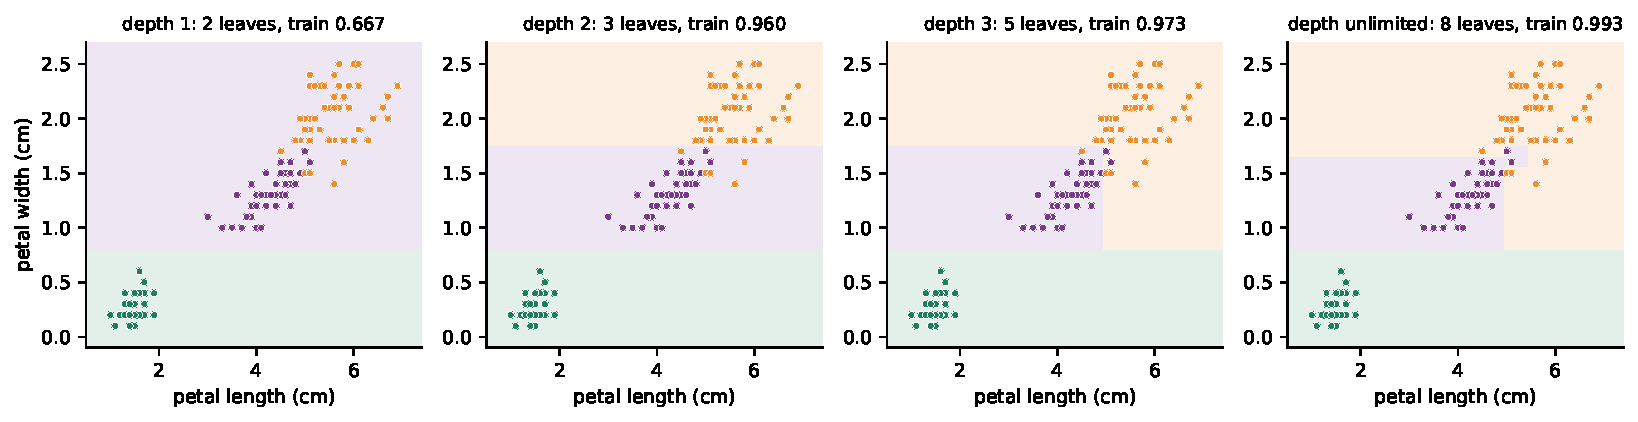
\includegraphics[width=0.98\textwidth]{partition.pdf}
  \caption{A decision tree is a recursive partition. Two features of
  \texttt{load\_iris}; the shaded regions are what the tree predicts. Each
  extra level of depth adds cuts, always parallel to an axis, always inside a
  region an earlier cut produced. Depth 1 separates one species perfectly;
  depth 2 gets to $0.960$ training accuracy with three leaves; unlimited depth
  reaches $0.993$ with eight, and the extra leaves are the two overlapping
  species being carved apart one point at a time.}
  \label{fig:partition}
\end{figure}

Read the last panel carefully. The thin slivers on the right are what
overfitting looks like geometrically: regions drawn around individual training
points. Cross-validated, depth 2 scores $0.9267$ and the unlimited tree also
scores $0.9267$ --- all that extra structure bought nothing.

\subsection{Induction is greedy, and it has to be}

Building the tree means choosing which question goes at the root, which goes
below each branch, and so on. There are astronomically many trees consistent
with a given table, and finding the smallest one is NP-complete. So every
practical algorithm is \textbf{greedy}: pick the single best question now, split
the data, and recurse on each part, never reconsidering an earlier choice.
This family of methods is called \textbf{top-down induction of decision trees}.

The only thing left to decide is what ``best question'' means. That is what an
\textbf{attribute selection measure} is, and Han, Kamber and Pei give three of
them: \textbf{information gain} (used by ID3), \textbf{gain ratio} (used by
C4.5) and the \textbf{Gini index} (used by CART). All three are in this
lecture. Information gain comes first, because the other two are best
understood as answers to problems it has.

\subsection{The running example}
\label{sec:table}

Everything is developed on one table: Quinlan's fourteen-day weather record,
the standard worked example for ID3 in every textbook and every examination.
Build it yourself rather than downloading it.

\begin{lstlisting}
COLS = ["Day", "Outlook", "Temperature", "Humidity", "Wind", "PlayTennis"]
TENNIS = [
    ("D1",  "Sunny",    "Hot",  "High",   "Weak",   "No"),
    ("D2",  "Sunny",    "Hot",  "High",   "Strong", "No"),
    ("D3",  "Overcast", "Hot",  "High",   "Weak",   "Yes"),
    ...
    ("D14", "Rain",     "Mild", "High",   "Strong", "No"),
]
\end{lstlisting}
\begin{codeout}
Day  Outlook   Temperature  Humidity Wind    PlayTennis
D1   Sunny     Hot          High    Weak    No
D2   Sunny     Hot          High    Strong  No
D3   Overcast  Hot          High    Weak    Yes
D4   Rain      Mild         High    Weak    Yes
D5   Rain      Cool         Normal  Weak    Yes
D6   Rain      Cool         Normal  Strong  No
D7   Overcast  Cool         Normal  Strong  Yes
D8   Sunny     Mild         High    Weak    No
D9   Sunny     Cool         Normal  Weak    Yes
D10  Rain      Mild         Normal  Weak    Yes
D11  Sunny     Mild         Normal  Strong  Yes
D12  Overcast  Mild         High    Strong  Yes
D13  Overcast  Hot          Normal  Weak    Yes
D14  Rain      Mild         High    Strong  No
rows 14   Yes 9   No 5
Outlook      levels: Overcast, Rain, Sunny
Temperature  levels: Cool, Hot, Mild
Humidity     levels: High, Normal
Wind         levels: Strong, Weak
\end{codeout}

Four attributes, one class column, and a \texttt{Day} identifier that is
\emph{not} an attribute. Section~\ref{sec:gainratio} is about what happens
when you forget that.

\notesources{\AMLUnitVISources}

% =========================================================================
\section{Entropy, from first principles}
\label{sec:entropy}

\subsection{The question entropy answers}

Take a node of the tree holding some rows. If every row has the same label,
the node is \textbf{pure} and there is nothing left to learn there. If the
labels are evenly split, the node is as \textbf{impure} as it can be, and
knowing which node a row landed in tells you nothing about its label. We need
a number that is $0$ in the first case, maximal in the second, and smooth in
between.

Shannon's answer, for a node whose class proportions are
$p_1, p_2, \dots, p_m$, is
\begin{equation}
  \label{eq:entropy}
  H = -\sum_{i=1}^{m} p_i \log_2 p_i ,
  \qquad\text{with the convention } 0\log_2 0 = 0 .
\end{equation}
Han, Kamber and Pei write the same quantity $\mathrm{Info}(D)$ and call it the
\emph{expected information needed to classify a tuple in $D$}. Both names
appear in examination papers; they are the same formula.

\subsection{Why the logarithm, and why base two}

Think of it as a coding problem. You must send someone the label of a randomly
drawn row using yes/no questions. If a label has probability $p$, an efficient
code gives it $\log_2 (1/p) = -\log_2 p$ bits: a label that occurs half the
time deserves one bit, a label that occurs an eighth of the time deserves
three. Equation~\eqref{eq:entropy} is just the \emph{average} of those costs,
weighted by how often each label occurs. So $H$ is measured in \textbf{bits}
and means ``the average number of yes/no questions needed to pin down the
label of one row''.

Base two is a choice of unit, not of substance. Base $e$ gives \emph{nats} and
base ten gives \emph{hartleys}; every entropy in this lecture would be
multiplied by the same constant and every comparison between attributes would
come out the same. We use base two because the answers are then small readable
numbers and because ``one bit'' is a thing you can picture.

\begin{lstlisting}
for k in (2, 4, 8, 16):
    print(k, "equally likely messages ->", log2(k), "bits")
draws = rng.random(1000) < 0.9          # a biased source
p = draws.mean()
print(p, -(p*log2(p) + (1-p)*log2(1-p)))
\end{lstlisting}
\begin{codeout}
why base 2: H is the average number of yes/no questions per message
    2 equally likely messages -> log2(2) = 1.0 bits, and 1 yes/no questions do identify one
    4 equally likely messages -> log2(4) = 2.0 bits, and 2 yes/no questions do identify one
    8 equally likely messages -> log2(8) = 3.0 bits, and 3 yes/no questions do identify one
   16 equally likely messages -> log2(16) = 4.0 bits, and 4 yes/no questions do identify one
a biased two-class source, 1000 draws at p(Yes) = 0.9
   observed p(Yes) 0.9040   H 0.4562 bits per draw
   a naive 1-bit-per-draw code costs 1000 bits; the entropy bound is 456
\end{codeout}

The last two lines are the point of the whole definition. A stream of a
thousand labels that are $90\%$ ``Yes'' can be sent in $456$ bits rather than
$1000$, because it is predictable. \textbf{Entropy measures unpredictability,
and a node of a decision tree is exactly a place where we want the labels to be
predictable.}

\subsection{The two values you must know}

\begin{worked}[Entropy at the two extremes]
\textbf{A pure node.} All rows are ``Yes'', so $p_{\text{Yes}} = 1$ and
$p_{\text{No}} = 0$:
\[
  H = -1\log_2 1 - 0\log_2 0 = -1 \times 0 - 0 = \mathbf{0}.
\]
No questions are needed. You already know the answer.

\textbf{An evenly split binary node.} $p_{\text{Yes}} = p_{\text{No}} = 1/2$:
\[
  H = -\tfrac12 \log_2 \tfrac12 - \tfrac12 \log_2 \tfrac12
    = -\tfrac12(-1) - \tfrac12(-1) = \mathbf{1} \text{ bit}.
\]
Exactly one yes/no question is needed, which is obviously right.

\textbf{$m$ equally likely classes.} $p_i = 1/m$ for every $i$, so
\[
  H = -\sum_{i=1}^m \tfrac1m \log_2 \tfrac1m = \log_2 m .
\]
Three classes give $1.5850$ bits, four give $2$, ten give $3.3219$. This is the
ceiling: no node with $m$ classes can have entropy above $\log_2 m$.
\end{worked}

\begin{lstlisting}
def H(p):
    return 0.0 if p in (0.0, 1.0) else -(p*log2(p) + (1-p)*log2(1-p))
for p in (0.0, 0.25, 1/3, 0.5, 0.75, 1.0):
    print(p, H(p))
\end{lstlisting}
\begin{codeout}
entropy of a two-class node, H(p) = -p log2 p - (1-p) log2 (1-p)
   p = 0.0000    H = 0.0000  pure
   p = 0.0500    H = 0.2864
   p = 0.1000    H = 0.4690
   p = 0.2500    H = 0.8113
   p = 0.3333    H = 0.9183
   p = 0.5000    H = 1.0000  MAXIMUM
   p = 0.6667    H = 0.9183
   p = 0.7500    H = 0.8113
   p = 0.9000    H = 0.4690
   p = 1.0000    H = 0.0000  pure
uniform over k classes: H = log2(k)
   k =  2   H = 1.0000   log2(k) = 1.0000
   k =  3   H = 1.5850   log2(k) = 1.5850
   k =  4   H = 2.0000   log2(k) = 2.0000
   k =  8   H = 3.0000   log2(k) = 3.0000
   k = 10   H = 3.3219   log2(k) = 3.3219
\end{codeout}

\begin{figure}[tb]
  \centering
  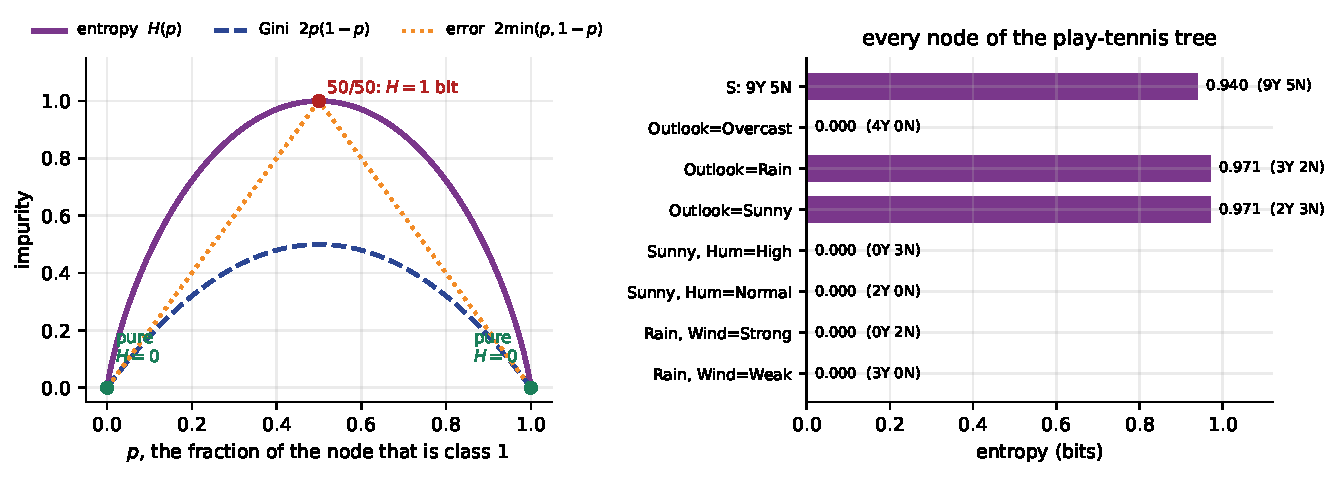
\includegraphics[width=0.94\textwidth]{entropy.pdf}
  \caption{Left: the binary entropy $H(p)$, with the Gini index and the
  misclassification error rescaled to peak at the same height. All three are
  zero at $p=0$ and $p=1$ and maximal at $p=\tfrac12$; entropy is the tallest
  and error the most sharply pointed, which is why the error rate makes a poor
  splitting criterion --- it is flat where the others still discriminate.
  Right: every node of the play-tennis tree built in
  Section~\ref{sec:worked}, in the order it is created. The root is at
  $0.9403$, two children at $0.9710$, and every one of the five leaves is
  exactly $0$.}
  \label{fig:entropy}
\end{figure}

\begin{caution}
$H(p)$ is symmetric: a node with $9$ Yes and $5$ No has exactly the same
entropy as one with $5$ Yes and $9$ No. Entropy measures \emph{how mixed}, not
\emph{which class dominates}. Two nodes with the same entropy can predict
opposite labels.
\end{caution}

\notesources{\AMLUnitVISources}

% =========================================================================
\section{Information gain, and the full worked calculation}
\label{sec:worked}

\subsection{The definition}

Splitting a set $S$ on attribute $A$ divides it into subsets
$S_{v_1}, \dots, S_{v_k}$, one per value of $A$. The impurity that survives
the split is the \emph{weighted average} of the children's entropies, each
child weighted by the fraction of rows it received:
\begin{equation}
  \label{eq:infoA}
  \mathrm{Info}_A(S) \;=\; \sum_{v \in \mathrm{values}(A)}
    \frac{|S_v|}{|S|} \, H(S_v) .
\end{equation}
The \textbf{information gain} is what the split removed:
\begin{equation}
  \label{eq:gain}
  \mathrm{Gain}(S, A) \;=\; H(S) - \mathrm{Info}_A(S) .
\end{equation}
ID3 chooses the attribute with the largest gain. Two facts make that a
sensible rule. First, $\mathrm{Gain} \ge 0$ always: splitting cannot increase
the weighted average entropy. Second, $\mathrm{Gain}(S,A) = H(S)$ exactly when
every child is pure --- the split has answered the question completely.

\begin{keyidea}
Information gain is the number of bits of uncertainty about the class that
asking about $A$ removes. Choosing the attribute of largest gain is choosing
the question that tells you the most.
\end{keyidea}

\subsection{Step 1: the entropy of the whole table}

\begin{worked}[$H(S)$ for the fourteen days]
Nine of the fourteen days are ``Yes'' and five are ``No'', so
$p_{\text{Yes}} = 9/14 = 0.642857$ and $p_{\text{No}} = 5/14 = 0.357143$.
\[
  H(S) = -\frac{9}{14}\log_2\frac{9}{14} - \frac{5}{14}\log_2\frac{5}{14} .
\]
The two logarithms are $\log_2 0.642857 = -0.637430$ and
$\log_2 0.357143 = -1.485427$, so
\[
  H(S) = 0.642857 \times 0.637430 + 0.357143 \times 1.485427
       = 0.409776 + 0.530510 = \mathbf{0.940286}\ \text{bits}.
\]
Sanity check: the maximum for two classes is $1$, and $9$ against $5$ is
close to even, so a value just under $1$ is what we should expect.
\end{worked}

\begin{lstlisting}
def entropy(rows):
    n = len(rows)
    return -sum((c/n) * log2(c/n) for c in class_counts(rows) if c)
print(entropy(TENNIS))
\end{lstlisting}
\begin{codeout}
S has 9 Yes and 5 No out of 14
H(S) = -(9/14)log2(9/14) - (5/14)log2(5/14)
     = -(0.642857)(-0.637430) - (0.357143)(-1.485427)
     = 0.409776 + 0.530510 = 0.940286 bits
Gini(S) = 1 - (9/14)^2 - (5/14)^2 = 0.459184
\end{codeout}

\subsection{Step 2: the gain of every attribute}

Now the same arithmetic four times. Take \texttt{Outlook} slowly and the other
three at speed.

\begin{worked}[$\mathrm{Gain}(S, \texttt{Outlook})$]
\texttt{Outlook} has three values and divides the fourteen rows $4/5/5$:
\begin{center}
\begin{tabular}{@{}lrrrl@{}}
\toprule
value & rows & Yes & No & entropy of that child\\
\midrule
\texttt{Overcast} & $4$ & $4$ & $0$ &
  $H = -1\log_2 1 = 0$ \quad (pure)\\
\texttt{Rain}     & $5$ & $3$ & $2$ &
  $H = -\tfrac35\log_2\tfrac35 - \tfrac25\log_2\tfrac25 = 0.970951$\\
\texttt{Sunny}    & $5$ & $2$ & $3$ &
  $H = -\tfrac25\log_2\tfrac25 - \tfrac35\log_2\tfrac35 = 0.970951$\\
\bottomrule
\end{tabular}
\end{center}
Note that the last two entropies are equal --- $2$ Yes out of $5$ and $3$ Yes
out of $5$ are equally mixed. Now the weighted average:
\[
  \mathrm{Info}_{\texttt{Outlook}}(S)
   = \frac{4}{14}(0) + \frac{5}{14}(0.970951) + \frac{5}{14}(0.970951)
   = \frac{10}{14} \times 0.970951 = 0.693536 .
\]
\[
  \boxed{\ \mathrm{Gain}(S, \texttt{Outlook}) = 0.940286 - 0.693536
   = \mathbf{0.246750}\ }
\]
\end{worked}

\begin{worked}[The other three attributes]
\textbf{\texttt{Temperature}} splits $4/4/6$:
\begin{align*}
  \texttt{Cool}\ (3\text{Y},1\text{N})&: H = 0.811278 &
  \texttt{Hot}\ (2\text{Y},2\text{N})&: H = 1.000000 &
  \texttt{Mild}\ (4\text{Y},2\text{N})&: H = 0.918296
\end{align*}
\[
  \mathrm{Info} = \tfrac{4}{14}(0.811278) + \tfrac{4}{14}(1.000000)
                + \tfrac{6}{14}(0.918296) = 0.911063,
  \qquad \mathrm{Gain} = \mathbf{0.029223}.
\]

\textbf{\texttt{Humidity}} splits $7/7$:
\begin{align*}
  \texttt{High}\ (3\text{Y},4\text{N})&: H = 0.985228 &
  \texttt{Normal}\ (6\text{Y},1\text{N})&: H = 0.591673
\end{align*}
\[
  \mathrm{Info} = \tfrac12(0.985228) + \tfrac12(0.591673) = 0.788450,
  \qquad \mathrm{Gain} = \mathbf{0.151836}.
\]

\textbf{\texttt{Wind}} splits $6/8$:
\begin{align*}
  \texttt{Strong}\ (3\text{Y},3\text{N})&: H = 1.000000 &
  \texttt{Weak}\ (6\text{Y},2\text{N})&: H = 0.811278
\end{align*}
\[
  \mathrm{Info} = \tfrac{6}{14}(1.000000) + \tfrac{8}{14}(0.811278)
                 = 0.892159,
  \qquad \mathrm{Gain} = \mathbf{0.048127}.
\]
\end{worked}

\begin{lstlisting}
def info_after(rows, attr):
    n = len(rows)
    return sum(len(sub)/n * entropy(sub) for _, sub in partition(rows, attr))
for a in ["Outlook", "Temperature", "Humidity", "Wind"]:
    print(a, info_after(TENNIS, a), entropy(TENNIS) - info_after(TENNIS, a))
\end{lstlisting}
\begin{codeout}
Information gain of Outlook, step by step
   Outlook = Overcast    4 rows  4 Yes 0 No   H = 0.000000
   Outlook = Rain        5 rows  3 Yes 2 No   H = 0.970951
   Outlook = Sunny       5 rows  2 Yes 3 No   H = 0.970951
   Info_Outlook(S) = (4/14)(0.0000) + (5/14)(0.9710) + (5/14)(0.9710)
                   = 0.693536
   Gain(S, Outlook) = 0.940286 - 0.693536 = 0.246750
\end{codeout}
\begin{codeout}
attribute      Info_A(S)     Gain     rank
Outlook        0.693536   0.246750   1
Temperature    0.911063   0.029223   4
Humidity       0.788450   0.151836   2
Wind           0.892159   0.048127   3
ID3 splits the root on Outlook
runner-up Humidity is behind by 0.094914
\end{codeout}

\begin{figure}[tb]
  \centering
  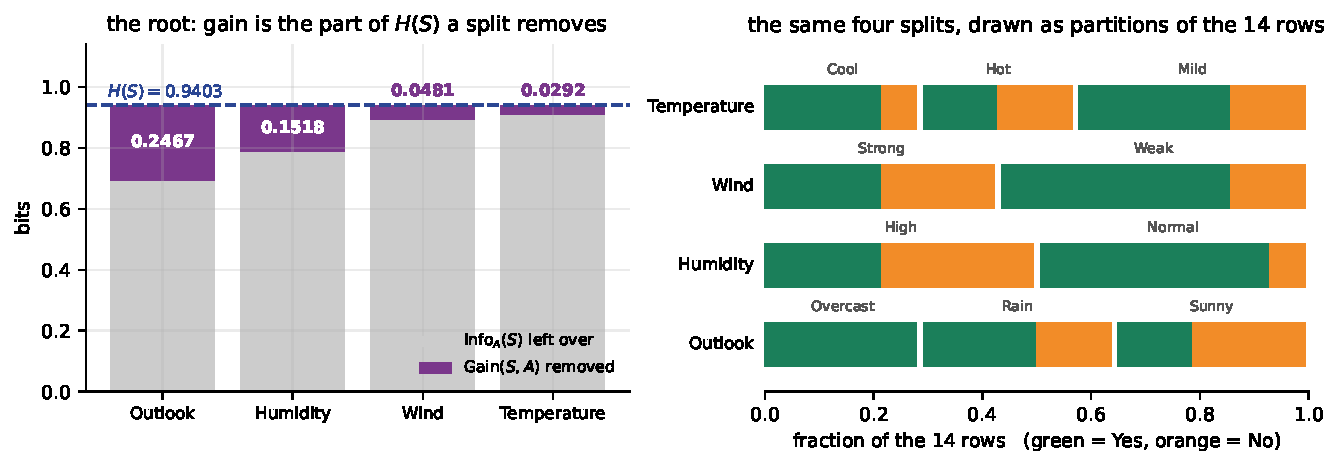
\includegraphics[width=0.98\textwidth]{tennisgain.pdf}
  \caption{Left: each bar is $H(S) = 0.9403$ split into the part a question
  about that attribute removes (purple, the gain) and the part it leaves
  behind (grey, $\mathrm{Info}_A(S)$). Right: the same four splits drawn as
  partitions of the fourteen rows, green for Yes and orange for No. Look at
  the \texttt{Outlook} row: the \texttt{Overcast} block is entirely green,
  which is where its gain comes from. Look at the \texttt{Temperature} row:
  every block is a mixture, which is why its gain is $0.0292$.}
  \label{fig:tennisgain}
\end{figure}

\begin{keyidea}
\texttt{Outlook} wins with $0.2467$ bits, and the reason is visible in one
number: it is the only attribute with a \textbf{pure child}. Four
\texttt{Overcast} days, four ``Yes'', entropy $0$. An attribute earns gain by
producing children that are less mixed than the parent, and a pure child is
the most any child can contribute.
\end{keyidea}

\begin{caution}
Do not compare $\mathrm{Info}_A(S)$ across attributes and pick the largest ---
you want the \emph{smallest} $\mathrm{Info}$, equivalently the largest gain.
This sign error is the single commonest mistake in the examination, and it
gives \texttt{Temperature} as the winner, which is the worst of the four.
\end{caution}

\notesources{\AMLUnitVISources}

% =========================================================================
\section{The ID3 algorithm}
\label{sec:id3}

\subsection{The algorithm}

ID3 --- Iterative Dichotomiser 3, Quinlan 1986 --- is
Equations~\eqref{eq:infoA} and \eqref{eq:gain} applied recursively.

\begin{quote}
\textbf{ID3}$(S, \text{attributes})$
\begin{enumerate}[leftmargin=1.6em,itemsep=1pt]
  \item If every row of $S$ has the same class $c$, return a leaf labelled $c$.
  \item If \text{attributes} is empty, return a leaf labelled with the
    \textbf{majority} class of $S$.
  \item Otherwise let $A^\star = \arg\max_A \mathrm{Gain}(S, A)$.
  \item Create a node testing $A^\star$. For each value $v$ of $A^\star$:
    \begin{itemize}[leftmargin=1.2em,itemsep=0pt]
      \item let $S_v$ be the rows of $S$ with $A^\star = v$;
      \item if $S_v$ is empty, attach a leaf labelled with the majority class
        of $S$;
      \item otherwise attach
        \textbf{ID3}$(S_v, \text{attributes} \setminus \{A^\star\})$.
    \end{itemize}
  \item Return the node.
\end{enumerate}
\end{quote}

Three details matter. \textbf{An attribute is used at most once on any path},
because once you have split on it every row below has the same value and a
second split would be useless. \textbf{The split is multiway}: an attribute
with $k$ values produces $k$ branches, not two. And \textbf{ID3 does no
pruning at all} --- it grows until every leaf is pure or it runs out of
attributes, which is Section~\ref{sec:prune}'s problem.

\subsection{Step 3: recursing into the branches}

\begin{worked}[The \texttt{Sunny} branch]
The five \texttt{Sunny} days are D1, D2, D8 (No) and D9, D11 (Yes): two Yes
and three No, so $H = 0.970951$. \texttt{Outlook} is used up; three attributes
remain.
\begin{center}
\begin{tabular}{@{}llr@{}}
\toprule
attribute & the split & gain\\
\midrule
\texttt{Temperature} & \texttt{Hot}\,(0Y,2N), \texttt{Mild}\,(1Y,1N),
  \texttt{Cool}\,(1Y,0N) & $0.570951$\\
\texttt{Humidity} & \texttt{High}\,(0Y,3N), \texttt{Normal}\,(2Y,0N) &
  $\mathbf{0.970951}$\\
\texttt{Wind} & \texttt{Strong}\,(1Y,1N), \texttt{Weak}\,(1Y,2N) & $0.019973$\\
\bottomrule
\end{tabular}
\end{center}
\texttt{Humidity} scores $0.970951$, which is the \emph{entire} entropy of the
node --- both children are pure, so $\mathrm{Info} = 0$ and the branch is
finished in one step. Three high-humidity sunny days: no tennis. Two
normal-humidity sunny days: tennis.
\end{worked}

\begin{worked}[The \texttt{Rain} branch]
The five \texttt{Rain} days are D4, D5, D10 (Yes) and D6, D14 (No): three Yes
and two No, so again $H = 0.970951$.
\begin{center}
\begin{tabular}{@{}llr@{}}
\toprule
attribute & the split & gain\\
\midrule
\texttt{Temperature} & \texttt{Mild}\,(2Y,1N), \texttt{Cool}\,(1Y,1N) &
  $0.019973$\\
\texttt{Humidity} & \texttt{High}\,(1Y,1N), \texttt{Normal}\,(2Y,1N) &
  $0.019973$\\
\texttt{Wind} & \texttt{Strong}\,(0Y,2N), \texttt{Weak}\,(3Y,0N) &
  $\mathbf{0.970951}$\\
\bottomrule
\end{tabular}
\end{center}
\texttt{Wind} splits it perfectly. Rain and a strong wind: no tennis. Rain and
a weak wind: tennis. Note that \texttt{Temperature} and \texttt{Humidity} tie
at $0.019973$ here --- ties happen, and an implementation must break them
somehow, usually by attribute order.
\end{worked}

\begin{lstlisting}
def id3(rows, attrs):
    yes, no = counts(rows)
    if yes == 0 or no == 0:                 # pure -> leaf
        return Leaf("Yes" if yes else "No")
    if not attrs:                           # out of attributes -> majority
        return Leaf("Yes" if yes >= no else "No")
    best = max(attrs, key=lambda a: gain(rows, a))
    return Node(best, {v: id3(sub, [a for a in attrs if a != best])
                       for v, sub in partition(rows, best)})
\end{lstlisting}
\begin{codeout}
[9 Yes, 5 No  H=0.9403]  split on Outlook (gain 0.2467)
   Outlook=Overcast: [4 Yes, 0 No  H=0.0000] --> Yes
   Outlook=Rain: [3 Yes, 2 No  H=0.9710]  split on Wind (gain 0.9710)
      Wind=Strong: [0 Yes, 2 No  H=0.0000] --> No
      Wind=Weak: [3 Yes, 0 No  H=0.0000] --> Yes
   Outlook=Sunny: [2 Yes, 3 No  H=0.9710]  split on Humidity (gain 0.9710)
      Humidity=High: [0 Yes, 3 No  H=0.0000] --> No
      Humidity=Normal: [2 Yes, 0 No  H=0.0000] --> Yes
leaves: 5
\end{codeout}

\begin{figure}[tb]
  \centering
  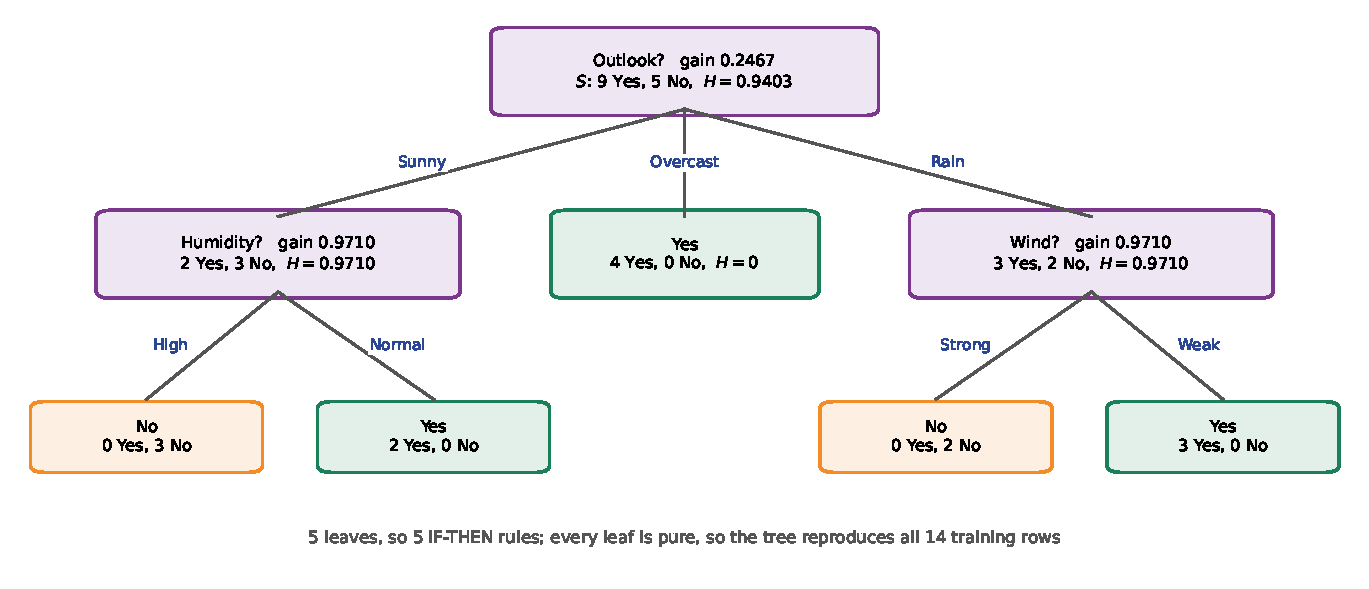
\includegraphics[width=0.98\textwidth]{tennistree.pdf}
  \caption{The tree ID3 builds on the fourteen-row table, with the class
  counts, the entropy and the winning gain at every node. Depth 2, five
  leaves, every leaf pure. \texttt{Temperature} never appears: its gain was
  the smallest at the root, and by the time each branch was reached another
  attribute had already separated it completely.}
  \label{fig:tennistree}
\end{figure}

\texttt{Temperature} not appearing in the final tree is worth a moment. It is
not that temperature is irrelevant to tennis; it is that, \emph{given} the
outlook, humidity and wind already account for these fourteen days. A greedy
algorithm answers ``what is the best question to ask next'', not ``which
variables matter''.

\subsection{Continuous attributes}
\label{sec:continuous}

ID3 as stated handles categorical attributes only. The C4.5 extension --- and
CART, and scikit-learn --- handles a numeric attribute by turning it into a
binary one: sort the distinct values, take the midpoint of each adjacent pair
as a candidate threshold $t$, and score the binary split
$x \le t$ against $x > t$ with the same formula. With $d$ distinct values
there are $d-1$ candidates, and the algorithm tries all of them.

\begin{lstlisting}
vals = np.unique(petal_length)
cands = (vals[:-1] + vals[1:]) / 2          # the midpoints
best = max(cands, key=lambda t: gain_of_threshold(t))
\end{lstlisting}
\begin{codeout}
a continuous attribute: where does the threshold come from?
   43 distinct petal-length values -> 42 candidate midpoints
   H(all 150 rows, setosa vs rest) = 0.918296
   best midpoint 2.45 cm, gain 0.918296  (a perfect split)
   scikit-learn's threshold: 2.45  -- the same number
\end{codeout}

Forty-two candidate thresholds, one of them perfect, and scikit-learn finds
the same $2.45$ cm. Note also that a numeric attribute can be split
\emph{again} further down the tree at a different threshold, unlike a
categorical one --- which is why \texttt{petal width} appears twice in the
iris tree of Section~\ref{sec:rules}.

\subsection{scikit-learn implements CART, not ID3}

This trips people up in the lab, so measure it. Give scikit-learn the same
fourteen rows, one-hot encoded because it cannot take strings, and ask for
\texttt{criterion="entropy"}.

\begin{lstlisting}
t = DecisionTreeClassifier(criterion="entropy", random_state=0).fit(X, y)
print(export_text(t, feature_names=names))
\end{lstlisting}
\begin{codeout}
|--- Outlook=Overcast <= 0.50
|   |--- Humidity=Normal <= 0.50
|   |   |--- Outlook=Rain <= 0.50
|   |   |   |--- class: 0
|   |   |--- Outlook=Rain >  0.50
|   |   |   |--- Wind=Strong <= 0.50
|   |   |   |   |--- class: 1
|   |   |   |--- Wind=Strong >  0.50
|   |   |   |   |--- class: 0
|   |--- Humidity=Normal >  0.50
|   |   |--- Wind=Weak <= 0.50
|   |   |   |--- Temperature=Cool <= 0.50
|   |   |   |   |--- class: 1
|   |   |   |--- Temperature=Cool >  0.50
|   |   |   |   |--- class: 0
|   |   |--- Wind=Weak >  0.50
|   |   |   |--- class: 1
depth 4, leaves 7, training accuracy 1.0000
our ID3 tree: depth 2, leaves 5, training accuracy 1.0000
root feature: Outlook=Overcast   (root impurity 0.940286, matches H(S) = 0.940286)
the binary questions available at the root, scored by information gain:
   Outlook=Overcast       gain 0.226000
   Humidity=Normal        gain 0.151836
   Humidity=High          gain 0.151836
   Outlook=Sunny          gain 0.102244
   Wind=Weak              gain 0.048127
the best BINARY question is Outlook=Overcast; the best 3-WAY question is Outlook
that is the whole difference: ID3 splits multiway, CART splits in two.
\end{codeout}

Depth 4 and seven leaves against our depth 2 and five. Both are perfect on the
training rows; they are simply different trees. The root impurity scikit-learn
reports is $0.940286$, which is our $H(S)$ exactly --- so the measure is
identical and only the \emph{shape} of the allowed split differs. Restricted
to binary questions, the best available is ``\texttt{Outlook = Overcast}?''
scoring $0.226000$, a little less than the three-way \texttt{Outlook} split's
$0.246750$, and the tree needs an extra level to recover the rest.

\begin{caution}
scikit-learn has no ID3 and no C4.5. It has an optimised CART, it always
splits in two, and it does not accept categorical columns --- you must encode
them. Do not report ``I ran ID3 in scikit-learn''. Say what you ran.
\end{caution}

\begin{tryit}
Fit \texttt{DecisionTreeClassifier(criterion="entropy", max\_depth=1)} on the
one-hot tennis table and print \texttt{tree\_.impurity[0]}. You should get
$0.940286$ --- the same $H(S)$ you computed with a pen in
Section~\ref{sec:worked}.
\end{tryit}

\notesources{\AMLUnitVISources}

% =========================================================================
\section{Converting a tree to rules}
\label{sec:rules}

A tree with $L$ leaves is exactly $L$ IF--THEN rules: walk from the root to
each leaf, conjoin the tests you passed through, and the leaf label is the
consequent. The rules are \textbf{mutually exclusive} (a row satisfies exactly
one) and \textbf{exhaustive} (every row satisfies one), because the leaves
partition the data.

\begin{worked}[The five rules of the tennis tree]
Reading Figure~\ref{fig:tennistree} left to right:
\begin{align*}
  R_1:\ &\textbf{IF } \texttt{Outlook} = \texttt{Overcast}
    &&\textbf{THEN } \texttt{PlayTennis} = \texttt{Yes} && (4\text{ rows})\\
  R_2:\ &\textbf{IF } \texttt{Outlook} = \texttt{Rain}
    \ \textbf{AND}\ \texttt{Wind} = \texttt{Strong}
    &&\textbf{THEN } \texttt{PlayTennis} = \texttt{No} && (2\text{ rows})\\
  R_3:\ &\textbf{IF } \texttt{Outlook} = \texttt{Rain}
    \ \textbf{AND}\ \texttt{Wind} = \texttt{Weak}
    &&\textbf{THEN } \texttt{PlayTennis} = \texttt{Yes} && (3\text{ rows})\\
  R_4:\ &\textbf{IF } \texttt{Outlook} = \texttt{Sunny}
    \ \textbf{AND}\ \texttt{Humidity} = \texttt{High}
    &&\textbf{THEN } \texttt{PlayTennis} = \texttt{No} && (3\text{ rows})\\
  R_5:\ &\textbf{IF } \texttt{Outlook} = \texttt{Sunny}
    \ \textbf{AND}\ \texttt{Humidity} = \texttt{Normal}
    &&\textbf{THEN } \texttt{PlayTennis} = \texttt{Yes} && (2\text{ rows})
\end{align*}
Five rules, nine conditions, $4+2+3+3+2 = 14$ rows. The rule set is the tree;
nothing has been added or lost.
\end{worked}

\begin{codeout}
one IF-THEN rule per root-to-leaf path
R1: IF Outlook = Overcast THEN PlayTennis = Yes      (4 rows)
R2: IF Outlook = Rain AND Wind = Strong THEN PlayTennis = No      (2 rows)
R3: IF Outlook = Rain AND Wind = Weak THEN PlayTennis = Yes      (3 rows)
R4: IF Outlook = Sunny AND Humidity = High THEN PlayTennis = No      (3 rows)
R5: IF Outlook = Sunny AND Humidity = Normal THEN PlayTennis = Yes      (2 rows)
rules: 5   conditions in total: 9
the rule set reproduces 14 of 14 training rows
\end{codeout}

\subsection{Why bother, if the rules are just the tree}

Three reasons, and they are Quinlan's.

\textbf{They read better.} ``If it is overcast, play'' is a sentence a
non-specialist can check against their own experience. A picture of a tree is
not.

\textbf{They can be simplified independently.} Once the rules are separate
objects, you can drop a condition from one of them without disturbing the
others --- something you cannot do to a tree, where removing a test removes the
whole subtree below it. C4.5's rule post-pruning does exactly this: for each
condition in each rule, ask whether removing it improves the rule's estimated
accuracy, and remove it if so.

\textbf{They can be reordered.} A rule set can be sorted by accuracy or by
coverage, with a default rule at the end, which often shortens it further.

\subsection{Rule simplification, measured}

Here is a real case. Fit a depth-3 tree to \texttt{load\_iris} and read out
the rules.

\begin{lstlisting}
ti = DecisionTreeClassifier(max_depth=3, random_state=0).fit(iris.data,
                                                            iris.target)
print(export_text(ti, feature_names=list(iris.feature_names)))
\end{lstlisting}
\begin{codeout}
leaves 5, so 5 rules; the tree scores 0.9733 on all 150 rows
R1: IF petal width (cm) <= 0.80 THEN setosa   (50 rows, impurity 0.000)
R2: IF petal width (cm) > 0.80 AND petal width (cm) <= 1.75
    AND petal length (cm) <= 4.95 THEN versicolor   (48 rows, impurity 0.041)
R3: IF petal width (cm) > 0.80 AND petal width (cm) <= 1.75
    AND petal length (cm) > 4.95 THEN virginica   (6 rows, impurity 0.444)
R4: IF petal width (cm) > 0.80 AND petal width (cm) > 1.75
    AND petal length (cm) <= 4.85 THEN virginica   (3 rows, impurity 0.444)
R5: IF petal width (cm) > 0.80 AND petal width (cm) > 1.75
    AND petal length (cm) > 4.85 THEN virginica   (43 rows, impurity 0.000)
R4 and R5 predict the SAME class, so the last condition can be dropped:
   IF petal width > 0.80 AND petal width > 1.75 THEN virginica  (46 rows)
rules before simplification 5, after 4
the 4 simplified rules still classify 146 of 150 iris rows correctly
\end{codeout}

$R_4$ and $R_5$ come from a split that separated three rows from forty-three
and then predicted \texttt{virginica} on both sides. The test on
\texttt{petal length} was worth some impurity to the splitter but nothing at
all to the prediction, so it can go. Four rules instead of five, and the same
$146$ of $150$ rows.

\begin{keyidea}
A leaf is a rule and a rule is a leaf, but the rule form is easier to prune,
because a condition can be deleted from one rule without touching any other.
That asymmetry is the whole reason C4.5 converts to rules before pruning.
\end{keyidea}

\begin{tryit}
Print the tennis tree's rules and check that the number of conditions equals
the number of edges on the root-to-leaf paths: $1 + 2 + 2 + 2 + 2 = 9$. Then
count the leaves in Figure~\ref{fig:tennistree}. Rules and leaves must always
be equal in number.
\end{tryit}

\notesources{\AMLUnitVISources}

% =========================================================================
\section{The Gini index, and how it compares}
\label{sec:gini}

\subsection{Definition}

CART does not use entropy. It uses the \textbf{Gini index}, the probability
that two rows drawn at random from the node have different labels:
\begin{equation}
  \label{eq:gini}
  \mathrm{Gini}(S) = 1 - \sum_{i=1}^{m} p_i^2 .
\end{equation}
Like entropy it is $0$ for a pure node and maximal for an even split, but its
maximum for two classes is $0.5$ rather than $1$, and it has no logarithm in
it --- which is why implementations like it. Gini gain is defined exactly as
before: the parent's index minus the weighted average of the children's.

\begin{worked}[Gini on the tennis table]
\[
  \mathrm{Gini}(S) = 1 - \Big(\tfrac{9}{14}\Big)^{\!2}
                       - \Big(\tfrac{5}{14}\Big)^{\!2}
    = 1 - 0.413265 - 0.127551 = \mathbf{0.459184}.
\]
For \texttt{Outlook}: $\mathrm{Gini}(\texttt{Overcast}) = 0$,
$\mathrm{Gini}(\texttt{Rain}) = 1 - 0.36 - 0.16 = 0.48$, and
$\mathrm{Gini}(\texttt{Sunny}) = 0.48$ as well, so
\[
  \mathrm{Gini}_{\texttt{Outlook}}(S)
   = \tfrac{4}{14}(0) + \tfrac{10}{14}(0.48) = 0.342857,
  \qquad \text{gain} = 0.459184 - 0.342857 = \mathbf{0.116327}.
\]
\end{worked}

\begin{codeout}
the same four attributes scored with the Gini index instead
Gini(S) = 0.459184
attribute      Gini_A(S)   Gini gain  rank   (entropy rank)
Outlook        0.342857    0.116327    1          1
Temperature    0.440476    0.018707    4          4
Humidity       0.367347    0.091837    2          2
Wind           0.428571    0.030612    3          3
entropy order: Outlook > Humidity > Wind > Temperature
Gini    order: Outlook > Humidity > Wind > Temperature
same winner? True      same full ordering? True
\end{codeout}

The numbers are all smaller --- Gini lives on a shorter scale --- but the
\emph{ranking is identical}, all four positions. That is the usual outcome and
it is why the choice of criterion is rarely the interesting decision.

\subsection{CART splits in two, so it must choose a subset}

There is one structural difference worth knowing. Because CART builds binary
trees, a three-valued attribute cannot produce three branches; the algorithm
must instead choose a \emph{subset} of the values to send left. With $k$
values there are $2^{k-1}-1$ distinct such cuts, since a subset and its
complement give the same partition.

\begin{codeout}
CART splits BINARY, so for a 3-valued attribute it must choose a subset
   {Overcast        } | rest    4 vs 10 rows   Gini gain 0.102041
   {Rain            } | rest    5 vs  9 rows   Gini gain 0.002041
   {Sunny           } | rest    5 vs  9 rows   Gini gain 0.065533
   (a subset and its complement are the same cut, so 3 values give 3 cuts)
   best binary cut on Outlook: {Overcast} | {Rain, Sunny}
   the 3-way multiway split ID3 uses scores 0.116327
\end{codeout}

The best binary cut scores $0.102041$ against the multiway split's $0.116327$.
Binary trees pay a little at each node and buy it back with depth.

\subsection{How often do they actually disagree?}

This is where you should be suspicious of textbook claims. ``Entropy and Gini
usually give the same tree'' is repeated everywhere; here is the measurement.

\begin{lstlisting}
# 2000 random tables, two competing categorical attributes each.
# This is a SWEEP: the point is the spread across 2000 different tables,
# so one stream, seeded once, supplies all of them.
rs = np.random.default_rng(0)            # the one seed for this lecture
contests = [random_table(rs) for _ in range(2000)]
same = sum((gain_e(A) > gain_e(B)) == (gain_g(A) > gain_g(B))
           for A, B in contests)
\end{lstlisting}
\begin{codeout}
   2-attribute contests on random tables : 1990 of 1999 agree  (99.55%)
   iris           root split: entropy f3<=0.8000   gini f3<=0.8000   same? True
   iris           5-fold accuracy  entropy 0.9333   gini 0.9333   difference +0.0000
   iris           on held-out rows the two trees agree on 97.78% of them
   wine           root split: entropy f6<=1.5750   gini f12<=755.0000   same? False
   wine           5-fold accuracy  entropy 0.9495   gini 0.9273   difference +0.0222
   wine           on held-out rows the two trees agree on 92.59% of them
   breast_cancer  root split: entropy f22<=105.9500   gini f20<=16.7950   same? False
   breast_cancer  5-fold accuracy  entropy 0.9384   gini 0.9262   difference +0.0122
   breast_cancer  on held-out rows the two trees agree on 92.98% of them
   200 bootstrap root splits of breast_cancer identical: 150 (75.0%)
   but the two stumps still label 98.40% of rows the same on average
\end{codeout}

\begin{figure}[tb]
  \centering
  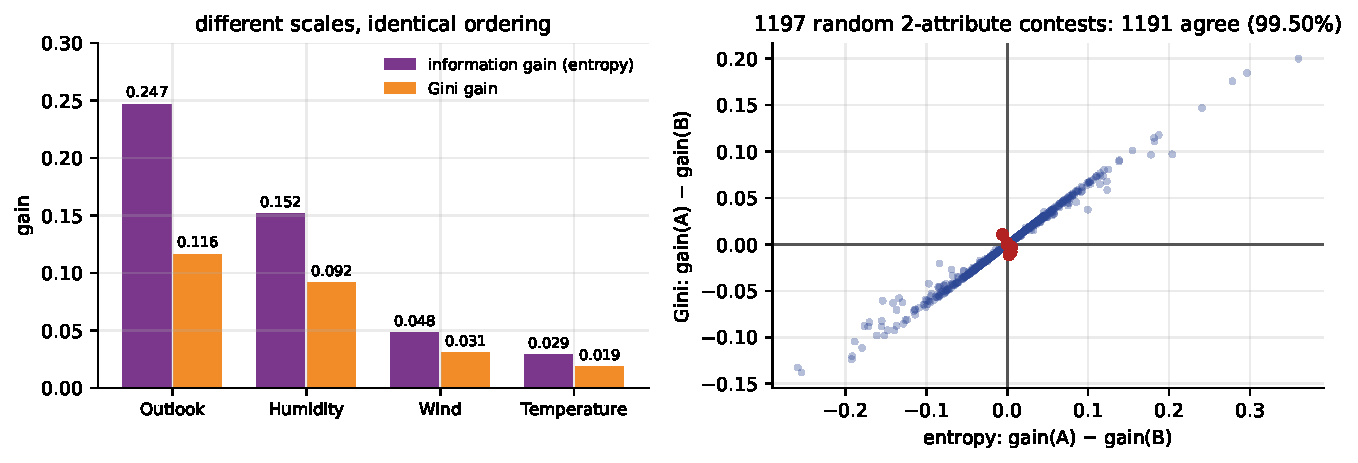
\includegraphics[width=0.94\textwidth]{giniig.pdf}
  \caption{Left: the four tennis attributes scored both ways. Different
  heights, identical ordering. Right: two thousand random two-attribute
  contests, entropy's margin on the horizontal axis against Gini's on the
  vertical. Almost every point is in the lower-left or upper-right quadrant,
  meaning the two measures agreed. The red points --- $0.45\%$ of them --- are
  the disagreements, and they all sit close to the origin, where the two
  attributes were nearly tied anyway.}
  \label{fig:giniig}
\end{figure}

Be precise about what these numbers say.

\textbf{When one attribute is clearly better, they agree.} $99.55\%$ of the
two-attribute contests, and every disagreement was a near-tie.

\textbf{When there are thousands of near-tied candidates, they often differ.}
On \texttt{breast\_cancer}, with $30$ features and hundreds of candidate
thresholds each, the root split differed on $25\%$ of bootstrap resamples ---
different feature, different threshold. That is a much larger number than the
folklore suggests.

\textbf{And it barely matters.} Those differing stumps still labelled $98.4\%$
of rows the same, the full trees agreed on $92$ to $98\%$ of held-out rows,
and the accuracy difference across three datasets was between $0.0000$ and
$0.0222$ --- in entropy's favour here, but well inside the noise of a
five-fold estimate.

\begin{keyidea}
Entropy and Gini are two measurements of the same thing, and they rank clearly
different attributes identically. They pick different splits when the
candidates are nearly tied, which on wide numeric data is often --- and when
they do, it makes almost no difference to the predictions. \textbf{Choose on
cost, not on principle: Gini has no logarithm and is the scikit-learn
default.}
\end{keyidea}

\begin{caution}
Do not compare an entropy gain with a Gini gain and conclude that one split is
better. $0.2467$ and $0.1163$ are the same split measured in different units.
Only compare gains computed with the same measure on the same node.
\end{caution}

\notesources{\AMLUnitVISources}

% =========================================================================
\section{Gain ratio, and the bias of information gain}
\label{sec:gainratio}

\subsection{The problem}

Information gain has a flaw, and it is not subtle. \textbf{It systematically
prefers attributes with many values.} An attribute that divides the data into
many small pieces will produce children that are purer almost by accident:
in the limit, an attribute with one value per row gives fourteen children of
one row each, every one of them pure, and a gain equal to the whole of $H(S)$.

The tennis table has such a column sitting right there in the file. It is
called \texttt{Day}.

\begin{worked}[Scoring the \texttt{Day} column]
\texttt{Day} has fourteen values in fourteen rows, so every child holds
exactly one row and has entropy $0$. Therefore
\[
  \mathrm{Info}_{\texttt{Day}}(S) = \sum_{v} \frac{1}{14}\times 0 = 0,
  \qquad
  \mathrm{Gain}(S, \texttt{Day}) = 0.940286 - 0 = \mathbf{0.940286} .
\]
That is the largest gain any attribute can possibly have, and it is
$0.940286 / 0.246750 = 3.81$ times \texttt{Outlook}'s. The Gini index has
exactly the same problem: Gini gain for \texttt{Day} is $0.459184$, the whole
of $\mathrm{Gini}(S)$.
\end{worked}

\begin{codeout}
now score the Day column, which is a row identifier
Day has 14 distinct values in 14 rows
   ... all 14 subsets have one row each, so every H = 0
Info_Day(S)  = 0.000000
Gain(S, Day) = 0.940286 - 0.000000 = 0.940286   <-- the largest possible
Gini gain(S, Day) = 0.459184   (Gini has exactly the same bias)
best real attribute:  Gain(S, Outlook) = 0.246750
Day beats it by a factor of 3.81
\end{codeout}

What does ID3 do with that? Exactly what it is told to.

\begin{codeout}
what happens if you let ID3 see the Day column
[9 Yes, 5 No  H=0.9403]  split on Day (gain 0.9403)
   Day=D1: [0 Yes, 1 No  H=0.0000] --> No
   Day=D10: [1 Yes, 0 No  H=0.0000] --> Yes
   Day=D11: [1 Yes, 0 No  H=0.0000] --> Yes
   ... (14 branches, one per row)
leaves 14, depth 1, conditions per rule 1
training rows reproduced: 14 of 14  (perfect)
a new row D15 (Sunny, Cool, Normal, Weak) matches 0 of the 14 rules
the 4-attribute tree classifies it as: Yes
\end{codeout}

\begin{keyidea}
A depth-1 tree with fourteen leaves, perfect on the training set, and
\textbf{it matches none of its own rules on a new day}. This is the cleanest
demonstration of overfitting in the whole course: a model that is right about
everything it has seen and has nothing whatever to say about anything else.
\end{keyidea}

\subsection{The fix: normalise by how much the split itself costs}

Quinlan's C4.5 divides the gain by the entropy of the \emph{split}, ignoring
the class labels entirely --- how many ways it divides the data and how
evenly:
\begin{equation}
  \label{eq:splitinfo}
  \mathrm{SplitInfo}_A(S) = -\sum_{v}\frac{|S_v|}{|S|}
     \log_2 \frac{|S_v|}{|S|},
  \qquad
  \mathrm{GainRatio}(S,A) = \frac{\mathrm{Gain}(S,A)}
                                 {\mathrm{SplitInfo}_A(S)} .
\end{equation}
A two-way even split has $\mathrm{SplitInfo} = 1$ and is not penalised at all.
A fourteen-way split has $\mathrm{SplitInfo} = \log_2 14 = 3.807$ and is
divided by nearly four.

\begin{worked}[Split information for the tennis attributes]
\begin{align*}
  \mathrm{SplitInfo}_{\texttt{Outlook}}
   &= -\tfrac{5}{14}\log_2\tfrac{5}{14} - \tfrac{4}{14}\log_2\tfrac{4}{14}
      - \tfrac{5}{14}\log_2\tfrac{5}{14} = 1.577406 \\
  \mathrm{SplitInfo}_{\texttt{Humidity}}
   &= -\tfrac{7}{14}\log_2\tfrac{7}{14} - \tfrac{7}{14}\log_2\tfrac{7}{14}
      = 1.000000 \\
  \mathrm{SplitInfo}_{\texttt{Day}} &= \log_2 14 = 3.807355
\end{align*}
so
$\mathrm{GainRatio}(\texttt{Outlook}) = 0.246750/1.577406 = 0.156428$,
$\mathrm{GainRatio}(\texttt{Humidity}) = 0.151836/1.000000 = 0.151836$,
and $\mathrm{GainRatio}(\texttt{Day}) = 0.940286/3.807355 = 0.246966$.
\end{worked}

\begin{codeout}
gain ratio = gain / split information
attribute      Gain      SplitInfo   GainRatio   gain rank  ratio rank
Outlook       0.246750   1.577406    0.156428      1          1
Temperature   0.029223   1.556657    0.018773      4          4
Humidity      0.151836   1.000000    0.151836      2          2
Wind          0.048127   0.985228    0.048849      3          3
information gain picks Outlook; gain ratio picks Outlook
\end{codeout}

Among the four genuine attributes, gain ratio changes nothing --- same winner,
same order. But look how close it came: \texttt{Outlook} at $0.156428$ against
\texttt{Humidity} at $0.151836$, a gap of $0.005$ where information gain had a
gap of $0.095$. The three-way split was penalised and the two-way one was not.

\subsection{Be honest: at fourteen rows the correction is not enough}

\begin{caution}[The textbook claim, checked]
Textbooks say gain ratio fixes the multi-valued bias. On this table it
\emph{reduces} it enormously but does not fix it:
$\mathrm{GainRatio}(\texttt{Day}) = 0.246966$ is still larger than
\texttt{Outlook}'s $0.156428$. The identifier would still be chosen.
Do not claim otherwise in an answer script.
\end{caution}

The correction is real, and it is large --- a $73.7\%$ cut, from $3.81\times$
the best real attribute down to $1.58\times$. It is simply not large enough at
$n = 14$, because $\log_2 14$ is only $3.8$. And that points straight at when
it \emph{is} enough: $\mathrm{SplitInfo}$ of an identifier is $\log_2 n$,
which grows with the table, while its gain is stuck at $H(S)$, which does not.

\begin{codeout}
the correction strengthens with cardinality: replicate the table
 copies  rows  Gain(RowID)  SplitInfo  GainRatio(RowID)  best real GR  Day wins?
      1    14     0.940286   3.807355          0.246966      0.156428   YES
      2    28     0.940286   4.807355          0.195593      0.156428   YES
      5    70     0.940286   6.129283          0.153409      0.156428   no
     10   140     0.940286   7.129283          0.131891      0.156428   no
     20   280     0.940286   8.129283          0.115667      0.156428   no
log2(rows) grows; the gain of a perfect identifier does not.
\end{codeout}

\begin{codeout}
the same run, but choosing the attribute by GAIN RATIO instead
   the 14-row table    gain picks Day (14 leaves)   gain ratio picks Day     (14 leaves)
   5 copies, 70 rows   gain picks Day (70 leaves)   gain ratio picks Outlook (5 leaves)
\end{codeout}

At seventy rows the picture is unambiguous. Information gain still builds the
useless seventy-leaf identifier tree; \textbf{gain ratio recovers the correct
five-leaf tree}. That is the result to remember, with the caveat about $n=14$
attached to it.

\begin{figure}[tb]
  \centering
  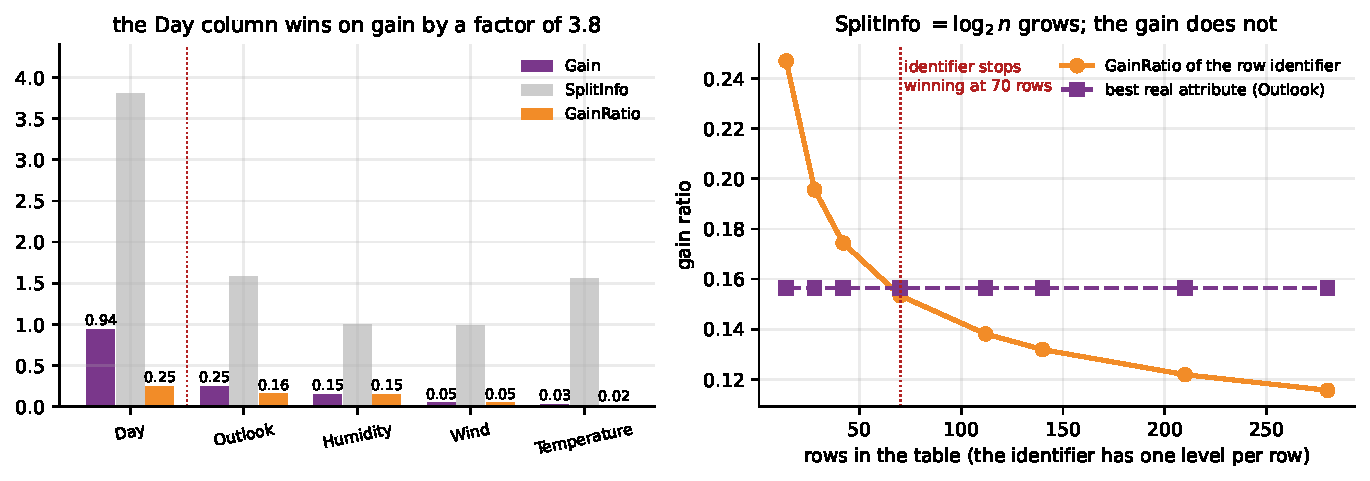
\includegraphics[width=0.96\textwidth]{gainratio.pdf}
  \caption{Left: gain, split information and gain ratio for the four real
  attributes and the \texttt{Day} identifier. \texttt{Day}'s gain bar is the
  tallest possible; its split-information bar is $3.807$, and dividing brings
  it down to $0.247$. Right: repeating the table so the identifier has more
  levels. Its gain ratio falls like $H(S)/\log_2 n$ while the best real
  attribute stays flat at $0.156$; they cross at seventy rows.}
  \label{fig:gainratio}
\end{figure}

Two further practical points. C4.5 does not use gain ratio blindly --- it
first discards any attribute whose plain gain is below the average, then
maximises the ratio among the rest, precisely because dividing by a tiny
$\mathrm{SplitInfo}$ can promote a useless near-constant attribute. And
scikit-learn implements neither: CART uses Gini or entropy, without
normalisation, and relies on binary splitting plus pruning to contain the
damage.

\begin{codeout}
the same identifier, one-hot encoded, given to scikit-learn
   4 attributes  (10 columns)     train 1.0000  depth 4  leaves 7  7-fold CV 0.6429
   + Day column  (24 columns)     train 1.0000  depth 3  leaves 5  7-fold CV 0.6429
   one-hot turns a 14-way question into 14 separate yes/no questions,
   so CART cannot isolate one row in a single split and the damage is
   milder than ID3's -- but the CV score is unchanged either way.
\end{codeout}

Report that honestly too: on fourteen rows the one-hot encoded identifier did
\emph{not} damage the cross-validated score, because a binary split on
``\texttt{Day = D7}?'' peels off one row rather than all fourteen. The
catastrophe in this section belongs to \emph{multiway} splitting on a
high-cardinality attribute. The lesson survives in either case, and it is the
short one: \textbf{drop identifier columns before you fit anything}.

\notesources{\AMLUnitVISources}

% =========================================================================
\section{Trees need no feature scaling}
\label{sec:scale}

Lecture 6 measured this from the other side: standardising the inputs changed
an RBF SVM's accuracy by $+0.0561$ and a decision tree's by exactly $0.0000$.
Here is why, and a stronger version of the demonstration.

Every question a tree asks is ``is $x_j \le t$?''. Apply any strictly
increasing function $g$ to column $j$. Then $x_j \le t$ if and only if
$g(x_j) \le g(t)$, so the \emph{same rows} go left --- with a different
threshold printed on the node. The set of partitions available to the
algorithm is unchanged, so the tree it finds is the same tree.

\begin{keyidea}
A split is a question about \textbf{order}, and a monotone transform preserves
order. Trees are therefore invariant to scaling, to $\log$, to any monotone
transform at all. Distance-based models are invariant to none of them, because
a distance is a question about \textbf{magnitude}.
\end{keyidea}

\begin{lstlisting}
for name, f in [("raw", lambda A: A),
                ("StandardScaler", sc.transform),
                ("log1p", np.log1p),
                ("cube", lambda A: A ** 3)]:
    t = DecisionTreeClassifier(random_state=0).fit(f(Xtr), ytr)
    print(name, t.get_n_leaves(), (t.predict(f(Xte)) == yte).mean())
\end{lstlisting}
\begin{codeout}
a tree needs no feature scaling: any increasing transform is a no-op
   tree  raw                              leaves 16 depth 6  test 0.906433  same predictions? True
   tree  StandardScaler                   leaves 16 depth 6  test 0.906433  same predictions? True
   tree  log1p (nonlinear, increasing)    leaves 16 depth 6  test 0.906433  same predictions? True
   tree  cube  (nonlinear, increasing)    leaves 16 depth 6  test 0.906433  same predictions? True
   tree  x -> -x (DECREASING)             leaves 19 depth 6  test 0.900585  same predictions? False
   contrast: a distance-based model on the same splits
   5-NN  raw                                                  test 0.912281
   5-NN  StandardScaler                                       test 0.947368
   5-NN  log1p (nonlinear, increasing)                        test 0.935673
   5-NN  cube  (nonlinear, increasing)                        test 0.918129
   spread of the 4 tree scores 0.0000    spread of the 4 5-NN scores 0.0351
\end{codeout}

Sixteen leaves, depth six, and \emph{identical predictions on every test row}
under an affine rescaling, a logarithm and a cube. Not ``similar'': identical.
The same four transforms move $5$-NN over a range of $0.0351$.

The fifth row is worth a sentence, because it looks like a counterexample.
Negating a column is also monotone, so the same partitions are available and
the tree should be equally good --- and it is, $0.9006$ against $0.9064$, one
extra test row. What changed is which of several \emph{equally good} splits
the greedy search happened to take first:

\begin{codeout}
   root feature raw 22 thr +106.1000 | negated 22 thr -106.1000 | same 2 groups? True
\end{codeout}

Same feature, mirrored threshold, and the root sends exactly the same rows
each way. The trees diverge lower down only through tie-breaking.

\begin{figure}[tb]
  \centering
  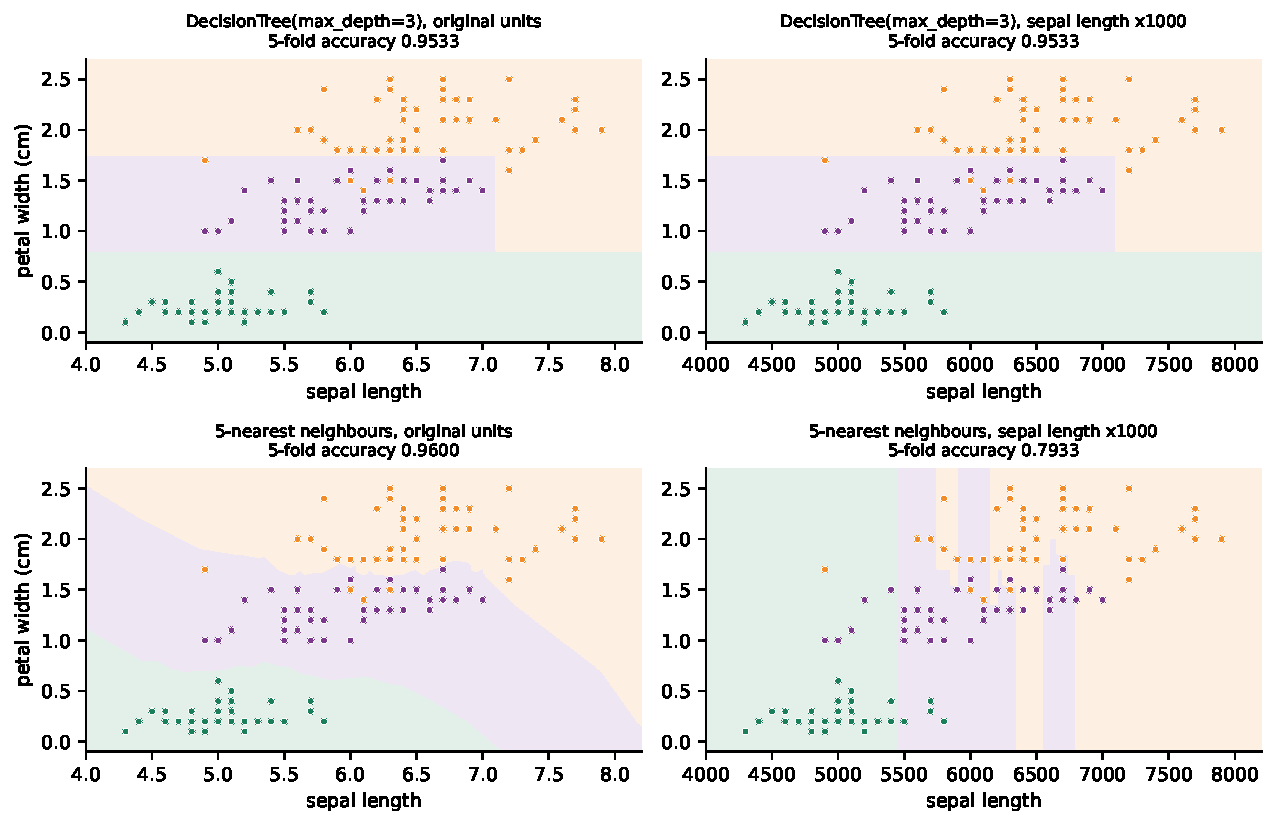
\includegraphics[width=0.86\textwidth]{invariance.pdf}
  \caption{Two features of \texttt{load\_iris}, with the right-hand column
  measuring sepal length in units a thousand times smaller. Top: the decision
  tree's regions are the \emph{same picture} --- the axis numbers changed and
  nothing else --- and the accuracy is $0.9533$ in both. Bottom: $5$-nearest
  neighbours collapses from $0.9600$ to $0.7933$, because sepal length now
  supplies essentially all of every distance and petal width has been switched
  off.}
  \label{fig:invariance}
\end{figure}

\begin{caution}
``Trees do not need scaling'' does not mean ``scaling a tree is wrong''. It is
a no-op, and it costs you something real: after scaling, the thresholds
printed on the nodes are no longer in the units of the problem, so nobody can
read the model. Leave a tree's inputs alone.

It also does \emph{not} extend to rotations. PCA before a tree mixes columns,
so the questions are no longer about single features and the invariance is
gone.
\end{caution}

\notesources{\AMLUnitVISources}

% =========================================================================
\section{Overfitting, and how to stop it}
\label{sec:prune}

\subsection{An unrestricted tree memorises}

ID3 and CART both stop only when a node is pure. On real data that means the
tree keeps splitting until it has carved out a region for each awkward
training row.

\begin{lstlisting}
Xtr, Xte, ytr, yte = train_test_split(Xb, yb, test_size=0.3,
                                      random_state=0, stratify=yb)
t = DecisionTreeClassifier(random_state=0).fit(Xtr, ytr)
print(t.get_depth(), t.get_n_leaves(), t.score(Xtr, ytr), t.score(Xte, yte))
\end{lstlisting}
\begin{codeout}
an unrestricted tree memorises the training set
   breast_cancer  398 train rows, 171 test rows
   unrestricted: depth 6  leaves 16  train 1.0000  test 0.9064  gap +0.0936
   leaves holding a single training row: 5 of 16
\end{codeout}
\begin{codeout}
a noisier problem, where the memorising is much more expensive
   600 rows, 20 features, 20% of the labels deliberately flipped
   unrestricted: depth 11  leaves 50  train 1.0000  test 0.6250  gap +0.3750
\end{codeout}

Training accuracy $1.0000$ in both cases. On \texttt{breast\_cancer} the price
is nine points; on a problem where a fifth of the labels are wrong \emph{by
construction} the price is thirty-seven. Five of the sixteen
\texttt{breast\_cancer} leaves hold a single patient each --- those are not
rules, they are copies.

\begin{keyidea}
A training accuracy of $1.0000$ from a decision tree is not an achievement.
An unpruned tree can always reach it as long as no two rows have identical
features and different labels. The only number worth reading is the held-out
one.
\end{keyidea}

\subsection{Pre-pruning: stop early}

Two dials, both arguments to \texttt{DecisionTreeClassifier}.
\texttt{max\_depth} caps how many questions a path may ask;
\texttt{min\_samples\_leaf} refuses to create a leaf holding fewer than a
stated number of rows. The tables below average over thirty random $70/30$
splits, because a single split of $569$ rows is far too noisy to choose a
hyper-parameter on.

\begin{codeout}
averaged over 30 random 70/30 splits of breast_cancer
max_depth   leaves   train    test     gap
   1           2.0   0.9275   0.8977   +0.0298
   2           4.0   0.9563   0.9199   +0.0364
   3           7.7   0.9750   0.9232   +0.0518
   4          11.2   0.9874   0.9263   +0.0610
   5          14.0   0.9946   0.9312   +0.0634
   6          15.8   0.9986   0.9277   +0.0709
   8          16.5   1.0000   0.9271   +0.0729
   10         16.5   1.0000   0.9271   +0.0729
   None       16.5   1.0000   0.9271   +0.0729
min_samples_leaf   leaves   train    test     gap
   1                 16.5   1.0000   0.9271   +0.0729
   2                 14.9   0.9904   0.9275   +0.0629
   5                 11.4   0.9757   0.9339   +0.0418
   10                 8.3   0.9607   0.9209   +0.0399
   20                 6.3   0.9438   0.9205   +0.0233
   50                 4.9   0.9275   0.8977   +0.0298
\end{codeout}
\begin{codeout}
the same two sweeps on the 20%-noise problem
   max_depth 1        2.0 leaves  train 0.7249  test 0.7067  gap +0.0183
   max_depth 2        4.0 leaves  train 0.7339  test 0.7035  gap +0.0304
   max_depth 3        7.8 leaves  train 0.7945  test 0.7291  gap +0.0654
   max_depth 4       14.2 leaves  train 0.8330  test 0.7380  gap +0.0951
   max_depth 6       32.1 leaves  train 0.9122  test 0.7157  gap +0.1965
   max_depth 8       48.2 leaves  train 0.9641  test 0.7093  gap +0.2549
   max_depth None    62.1 leaves  train 1.0000  test 0.6920  gap +0.3080
\end{codeout}

\begin{figure}[tb]
  \centering
  
\includegraphics[width=0.99\textwidth]{overfit.pdf}
  \caption{Training accuracy climbs monotonically with depth; test accuracy
  rises, peaks, and falls. On \texttt{breast\_cancer} the peak is shallow
  ($0.9312$ at depth 5 against $0.9271$ unrestricted) because the classes are
  well separated. On a problem with $20\%$ label noise it is dramatic:
  $0.7380$ at depth 4 against $0.6920$ unrestricted, and the gap between the
  two curves widens from $0.02$ to $0.31$. Right: \texttt{min\_samples\_leaf}
  is the same trade-off approached from the other end.}
  \label{fig:overfit}
\end{figure}

The shape is the bias--variance picture of Unit V in tree form. The
\emph{train--test gap} is the diagnostic: $+0.03$ at depth 1 and $+0.31$
unrestricted on the noisy problem. Watch the gap, not the training score.

\begin{caution}
Pre-pruning is greedy in the same way the tree is. A depth cap can stop a
branch just before the split that would have paid, and there is no way to know
that from inside the algorithm --- which is the standard argument for
\emph{post}-pruning: grow it all, then cut back with evidence.
\end{caution}

\subsection{Post-pruning: cost-complexity}

CART's method, and the one scikit-learn implements. For a tree $T$ define
\begin{equation}
  \label{eq:ccp}
  R_\alpha(T) = R(T) + \alpha\,|\widetilde{T}| ,
\end{equation}
where $R(T)$ is the tree's total impurity on the training data,
$|\widetilde{T}|$ is its number of leaves and $\alpha \ge 0$ is a price per
leaf. At $\alpha = 0$ the full tree wins. As $\alpha$ rises, whole subtrees
stop being worth their leaf count and collapse to a single node. The sequence
of trees produced as $\alpha$ increases is nested and finite, and
\texttt{cost\_complexity\_pruning\_path} returns the $\alpha$ values at which
it changes. You then \textbf{choose $\alpha$ by cross-validation}, exactly as
you would any other hyper-parameter.

\begin{lstlisting}
path = DecisionTreeClassifier(random_state=0
                              ).cost_complexity_pruning_path(Xtr, ytr)
for a in path.ccp_alphas[:-1]:
    print(a, cross_val_score(DecisionTreeClassifier(random_state=0,
                                                    ccp_alpha=a),
                             Xtr, ytr, cv=5).mean())
\end{lstlisting}
\begin{codeout}
cost-complexity pruning: R_alpha(T) = R(T) + alpha |leaves(T)|
   the path has 11 effective alphas, from 0.000000 to 0.026550
   alpha      leaves   train    5-fold CV   test
   0.002492     14   0.9975   0.9171      0.9064
   0.004902     10   0.9899   0.9121      0.9123
   0.008794      6   0.9774   0.9197      0.9181
   0.008992      5   0.9724   0.9197      0.9181
   0.019591      4   0.9623   0.9247      0.9006   <-- best CV
   0.025861      3   0.9322   0.9172      0.8889
   0.026550      2   0.9322   0.9172      0.8889
   chosen by cross-validation: alpha 0.019591, 4 leaves, test 0.9006
   unpruned: 16 leaves, test 0.9064
   pruning removed 12 of 16 leaves and changed the test score by -0.0058
   on breast_cancer the gain is in SIZE, not accuracy: report that.
\end{codeout}

\textbf{Report the result you got, not the one you wanted.} On
\texttt{breast\_cancer} cross-validation chose $\alpha = 0.0196$, which cut
the tree from sixteen leaves to four --- and cost $0.0058$ of test accuracy.
That is a real outcome and a defensible trade: a four-rule model a clinician
can read, for half a percentage point. But it is not the ``pruning improves
accuracy'' headline, and you should not pretend it is.

Where it does pay is where there is noise to stop fitting:

\begin{codeout}
the same procedure on the 20%-noise problem, where it does pay
   unpruned      :  50 leaves  train 1.0000  CV 0.6917  test 0.6250
   best CV alpha 0.013805:   8 leaves  train 0.8500  CV 0.7444  test 0.7000
   pruning removed 42 of 50 leaves and bought +0.0750 of test accuracy
\end{codeout}

Forty-two of fifty leaves removed and seven and a half points of test accuracy
gained. Same code, same procedure, different data.

\begin{figure}[tb]
  \centering
  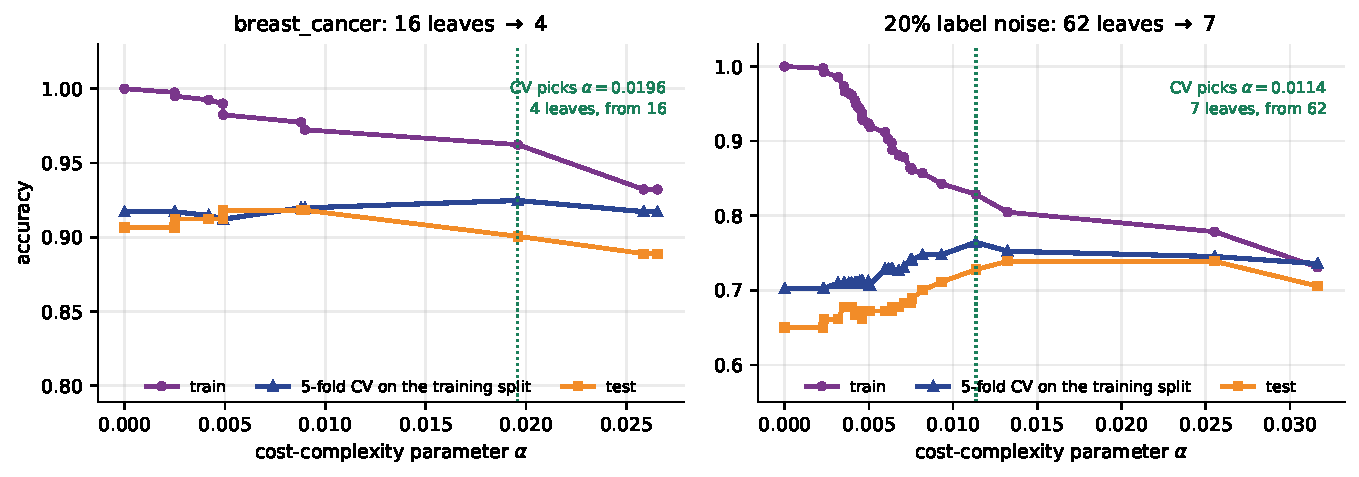
\includegraphics[width=0.94\textwidth]{ccp.pdf}
  \caption{The validation curve for cost-complexity pruning. Purple is
  training accuracy, which falls monotonically as $\alpha$ rises; blue is
  five-fold cross-validation \emph{on the training split}, which is what
  chooses $\alpha$; orange is the untouched test set. Left,
  \texttt{breast\_cancer}: the CV curve is nearly flat, so pruning buys size
  rather than accuracy. Right, $20\%$ label noise: the CV curve has a clear
  peak and following it takes the tree from $62$ leaves to $7$ and the test
  score from $0.625$ to $0.700$.}
  \label{fig:ccp}
\end{figure}

\begin{caution}
Choose $\alpha$ on cross-validation \emph{within the training split}, never on
the test set. The orange curve in Figure~\ref{fig:ccp} is drawn so that you
can see whether the procedure worked; it plays no part in choosing $\alpha$.
Picking the $\alpha$ that maximises the orange curve is the leakage error of
Lecture 6, and it will report an accuracy you cannot reproduce.
\end{caution}

\begin{tryit}
Run the \texttt{max\_depth} sweep on \texttt{load\_wine} instead. You should
find a shallower optimum than \texttt{breast\_cancer}'s --- $178$ rows and $13$
features leave much less room for depth. Report the train--test gap at each
depth as well as the accuracy.
\end{tryit}

\notesources{\AMLUnitVISources}

% =========================================================================
\section{Summary}

\begin{enumerate}[leftmargin=*]
  \item A decision tree is a nested set of IF--THEN rules built greedily,
    top-down, one question at a time. With numeric features it is a partition
    of the space into axis-parallel boxes.
  \item Entropy $H = -\sum p_i \log_2 p_i$ measures how mixed a node is, in
    bits. It is $\mathbf{0}$ for a pure node, $\mathbf{1}$ for an even binary
    split, and $\log_2 m$ for $m$ equally likely classes. Base two makes the
    unit a yes/no question; any other base rescales everything equally.
  \item On the fourteen-row play-tennis table, $H(S) = \mathbf{0.940286}$
    bits. The four information gains are \texttt{Outlook}
    $\mathbf{0.246750}$, \texttt{Humidity} $0.151836$, \texttt{Wind}
    $0.048127$, \texttt{Temperature} $0.029223$. \texttt{Outlook} wins because
    it is the only attribute with a pure child.
  \item Recursing, \texttt{Sunny} is split perfectly by \texttt{Humidity}
    (gain $0.970951$) and \texttt{Rain} perfectly by \texttt{Wind} (gain
    $0.970951$). The tree has depth 2, five leaves, and never uses
    \texttt{Temperature}.
  \item Five leaves means five IF--THEN rules, nine conditions, all fourteen
    training rows reproduced. On an iris tree, two rules predicting the same
    class allowed a condition to be dropped: five rules became four with the
    same $146$ of $150$ rows correct.
  \item The Gini index gives the identical ranking of the four attributes
    ($0.116327$ for \texttt{Outlook}), and entropy agreed with Gini on
    $\mathbf{99.55\%}$ of two thousand random contests. But on
    \texttt{breast\_cancer} the two chose different root splits on $25\%$ of
    bootstrap resamples --- and those stumps still labelled $98.4\%$ of rows
    identically. The choice of criterion is a cost decision, not a
    correctness one.
  \item Information gain is biased towards many-valued attributes. The
    \texttt{Day} column scores $\mathbf{0.940286}$, the maximum possible,
    $3.81\times$ \texttt{Outlook}, and ID3 given it builds a depth-1
    fourteen-leaf tree that is perfect on the training set and
    \textbf{matches none of its own rules on a new day}.
  \item Gain ratio divides by $\mathrm{SplitInfo} = \log_2 14 = 3.807$, a
    $73.7\%$ cut --- but at fourteen rows $0.246966$ still beats
    \texttt{Outlook}'s $0.156428$, so the identifier still wins. Replicate the
    table to seventy rows and gain ratio recovers the correct five-leaf tree
    while plain gain builds a seventy-leaf one.
  \item A tree is invariant to any monotone transform of a feature: raw,
    standardised, $\log$ and cubed all gave \textbf{identical predictions},
    $16$ leaves, test $0.906433$. The same four transforms moved $5$-NN over a
    range of $0.0351$, and multiplying one iris feature by $1000$ took $5$-NN
    from $0.9600$ to $0.7933$ while the tree stayed at $0.9533$.
  \item An unrestricted tree reaches training accuracy $\mathbf{1.0000}$
    every time. On \texttt{breast\_cancer} that costs $0.0936$ of test
    accuracy; with $20\%$ label noise it costs $0.3750$.
  \item Pre-pruning: the best \texttt{max\_depth} was $5$ on
    \texttt{breast\_cancer} ($0.9312$ against $0.9271$) and $4$ on the noisy
    problem ($0.7380$ against $0.6920$). \texttt{min\_samples\_leaf} $=5$ gave
    $0.9339$.
  \item Post-pruning: cost-complexity with $\alpha$ chosen by cross-validation
    cut \texttt{breast\_cancer} from $16$ leaves to $4$ for $-0.0058$ of
    accuracy, and the noisy tree from $50$ leaves to $8$ for
    $\mathbf{+0.0750}$. Report both kinds of result.
\end{enumerate}

% =========================================================================
\section{Practice questions}

Attempt these before reading Section~\ref{sec:solutions}. Questions 1, 2, 3
and 6 are pure hand arithmetic and are the ones most likely to appear on a
paper.

\begin{enumerate}[leftmargin=*]
  \item\label{q:entropy} A node contains $12$ rows: $9$ of class A and $3$ of
    class B. (a) Compute its entropy in bits, showing both terms. (b) Compute
    its Gini index. (c) A second node has $6$ of A and $6$ of B --- give both
    measures without a calculator. (d) A third has $12$ of A and $0$ of B ---
    same. (e) State the maximum entropy a node with four equally likely
    classes can have.

  \item\label{q:gain} A training set $S$ of $20$ rows has $12$ positive and
    $8$ negative examples. An attribute $A$ with values
    $a_1, a_2, a_3$ splits it as follows: $a_1$ gets $8$ rows ($6$P, $2$N),
    $a_2$ gets $6$ rows ($6$P, $0$N), $a_3$ gets $6$ rows ($0$P, $6$N).
    (a) Compute $H(S)$. (b) Compute the entropy of each child. (c) Compute
    $\mathrm{Info}_A(S)$ and $\mathrm{Gain}(S,A)$. (d) Compute
    $\mathrm{SplitInfo}_A(S)$ and the gain ratio. (e) An attribute $B$ splits
    the same $S$ into two halves of $10$, one with $9$P$1$N and one with
    $3$P$7$N. Which attribute does ID3 choose, and which does C4.5 choose?

  \item\label{q:tennis} Using the fourteen-row play-tennis table of
    Section~\ref{sec:table}, and \emph{without} looking at
    Section~\ref{sec:worked}: (a) compute $H(S)$; (b) compute
    $\mathrm{Gain}(S, \texttt{Humidity})$ showing the two child entropies;
    (c) compute $\mathrm{Gain}(S, \texttt{Wind})$; (d) state which of the four
    attributes ID3 puts at the root and by what margin over the runner-up;
    (e) explain in one sentence what \texttt{Outlook} has that the others do
    not.

  \item\label{q:recurse} Continue question~\ref{q:tennis}. (a) List the five
    \texttt{Sunny} rows with their labels and compute the entropy of that
    node. (b) Compute the information gain of \texttt{Humidity} and of
    \texttt{Wind} on those five rows. (c) Why is the winning gain here equal
    to the node's entropy? (d) Draw the completed tree. (e) Why does
    \texttt{Temperature} appear nowhere in it, and does that mean temperature
    is irrelevant to playing tennis?

  \item\label{q:rules} Write out the tree of question~\ref{q:recurse} as
    IF--THEN rules. (a) How many rules, and how many conditions in total?
    (b) Classify the new day (\texttt{Outlook}=\texttt{Rain},
    \texttt{Temperature}=\texttt{Hot}, \texttt{Humidity}=\texttt{Normal},
    \texttt{Wind}=\texttt{Strong}) and name the rule that fired. (c) Why is
    exactly one rule guaranteed to fire? (d) Give one advantage the rule form
    has over the tree form.

  \item\label{q:day} A colleague adds the \texttt{Day} column to the attribute
    list. (a) Compute $\mathrm{Gain}(S, \texttt{Day})$ by hand --- you should
    not need a calculator for $\mathrm{Info}_{\texttt{Day}}(S)$. (b) Compute
    $\mathrm{SplitInfo}_{\texttt{Day}}(S)$ and the gain ratio. (c) Describe
    the tree ID3 builds and its training accuracy. (d) What does that tree
    predict for a fifteenth day? (e) Does gain ratio fix the problem on
    \emph{this} table? Answer with the two numbers.

  \item\label{q:gini} A binary-class node has $p$ positive. (a) Show that
    $\mathrm{Gini} = 2p(1-p)$. (b) Show that both entropy and Gini are zero at
    $p=0$ and $p=1$ and maximal at $p=\tfrac12$, and give both maxima.
    (c) A node has $40$ rows, $30$ positive. Compute both measures.
    (d) Given the measured agreement in Section~\ref{sec:gini}, would you
    expect changing \texttt{criterion} from \texttt{"gini"} to
    \texttt{"entropy"} to change your accuracy much? Cite a number.

  \item\label{q:scale} You are told that a colleague standardised all $30$
    features of \texttt{breast\_cancer} before fitting a decision tree, and
    that this is why their accuracy is good. (a) What accuracy change should
    standardising have produced, and why? (b) Give the general statement about
    which transformations leave a tree unchanged. (c) Name one transformation
    that does \emph{not}, and say why. (d) Give one concrete reason not to
    scale a tree's inputs.

  \item\label{q:overfit} A student reports a decision tree with training
    accuracy $1.0000$ on a medical dataset and asks whether the model is
    ready to deploy. (a) What single number do you ask for, and what would
    worry you? (b) Name the two pre-pruning parameters and say what each
    controls. (c) Write the cost-complexity objective and say what $\alpha$
    prices. (d) Describe, in the correct order, how to choose $\alpha$
    properly. (e) What mistake produces an optimistic answer here?

  \item\label{q:design} You must build a readable model that predicts whether
    a loan application will default. The table has $50{,}000$ rows: an
    application ID, six numeric columns whose scales differ by four orders of
    magnitude, a three-level ordinal column, a nominal column with $40$
    levels, and a binary target with $6\%$ defaults. Design the approach.
    For each decision cite a measured number from this lecture.
\end{enumerate}

% =========================================================================
\section{Solutions}
\label{sec:solutions}

\textbf{1.} (a) $p_A = 9/12 = 0.75$, $p_B = 0.25$.
\[
  H = -0.75\log_2 0.75 - 0.25\log_2 0.25
    = 0.75(0.415037) + 0.25(2) = 0.311278 + 0.5 = 0.811278 .
\]
(b) $\mathrm{Gini} = 1 - 0.75^2 - 0.25^2 = 1 - 0.5625 - 0.0625 = 0.375$.

(c) Even split: $H = 1$ bit exactly, $\mathrm{Gini} = 1 - 0.25 - 0.25 = 0.5$,
both at their two-class maxima.

(d) Pure: $H = 0$, $\mathrm{Gini} = 0$.

(e) $\log_2 4 = 2$ bits.

\begin{codeout}
   p = 0.7500    H = 0.8113
   p = 0.5000    H = 1.0000  MAXIMUM
   p = 1.0000    H = 0.0000  pure
   k =  4   H = 2.0000   log2(k) = 2.0000
Gini(9A 3B) = 0.375   Gini(6A 6B) = 0.5   Gini(12A 0B) = 0.0
\end{codeout}

\medskip
\textbf{2.} (a) $p = 12/20 = 0.6$, so
$H(S) = -0.6\log_2 0.6 - 0.4\log_2 0.4 = 0.442179 + 0.528771 = 0.970951$.

(b) $a_1$ is $6$P$2$N, i.e.\ $p = 0.75$, so $H = 0.811278$. $a_2$ is pure,
$H = 0$. $a_3$ is pure, $H = 0$.

(c) $\mathrm{Info}_A(S) = \tfrac{8}{20}(0.811278) + \tfrac{6}{20}(0)
+ \tfrac{6}{20}(0) = 0.324511$, so
$\mathrm{Gain}(S,A) = 0.970951 - 0.324511 = \mathbf{0.646440}$.

(d) The split is $8/6/6$ out of $20$, i.e.\ proportions $0.4, 0.3, 0.3$:
\[
  \mathrm{SplitInfo}_A = -0.4\log_2 0.4 - 2(0.3\log_2 0.3)
   = 0.528771 + 2(0.521090) = 1.570951,
\]
so the gain ratio is $0.646440/1.570951 = \mathbf{0.411497}$.

(e) $B$'s children: $9$P$1$N has $H = 0.468996$; $3$P$7$N has $H = 0.881291$.
$\mathrm{Info}_B = \tfrac12(0.468996) + \tfrac12(0.881291) = 0.675143$, so
$\mathrm{Gain}(S,B) = 0.295808$ and, since $\mathrm{SplitInfo}_B = 1$, the
gain ratio is also $0.295808$. \textbf{Both algorithms choose $A$}: it wins on
gain ($0.6464$ against $0.2958$) and on gain ratio ($0.4115$ against
$0.2958$). Splitting into more parts did not save $B$.

\medskip
\textbf{3.} (a) $9$ Yes, $5$ No, so $H(S) = 0.940286$ (worked in
Section~\ref{sec:worked}).

(b) \texttt{Humidity} splits $7/7$. \texttt{High} is $3$Y$4$N:
$H = -\tfrac37\log_2\tfrac37 - \tfrac47\log_2\tfrac47 = 0.985228$.
\texttt{Normal} is $6$Y$1$N:
$H = -\tfrac67\log_2\tfrac67 - \tfrac17\log_2\tfrac17 = 0.591673$.
$\mathrm{Info} = \tfrac12(0.985228 + 0.591673) = 0.788450$ and
$\mathrm{Gain} = \mathbf{0.151836}$.

(c) \texttt{Wind} splits $6/8$. \texttt{Strong} is $3$Y$3$N, $H = 1$;
\texttt{Weak} is $6$Y$2$N, $H = 0.811278$.
$\mathrm{Info} = \tfrac{6}{14}(1) + \tfrac{8}{14}(0.811278) = 0.892159$,
$\mathrm{Gain} = \mathbf{0.048127}$.

(d) \texttt{Outlook}, at $0.246750$, ahead of \texttt{Humidity} by
$0.246750 - 0.151836 = \mathbf{0.094914}$.

(e) It is the only one with a \emph{pure child}: all four \texttt{Overcast}
days are ``Yes'', contributing entropy $0$ to the weighted average.

\medskip
\textbf{4.} (a) D1 (No), D2 (No), D8 (No), D9 (Yes), D11 (Yes) --- two Yes and
three No, so
$H = -\tfrac25\log_2\tfrac25 - \tfrac35\log_2\tfrac35 = 0.970951$.

(b) \texttt{Humidity}: \texttt{High} is D1, D2, D8, all No, $H = 0$;
\texttt{Normal} is D9, D11, both Yes, $H = 0$. So $\mathrm{Info} = 0$ and
$\mathrm{Gain} = \mathbf{0.970951}$. \texttt{Wind}: \texttt{Strong} is D2 (No)
and D11 (Yes), $H = 1$; \texttt{Weak} is D1, D8 (No) and D9 (Yes),
$H = 0.918296$. $\mathrm{Info} = \tfrac25(1) + \tfrac35(0.918296) = 0.950978$,
$\mathrm{Gain} = 0.019973$.

(c) Because $\mathrm{Gain} = H(S_v) - \mathrm{Info}$ and $\mathrm{Info} = 0$
when every child is pure. A gain equal to the node's entropy is the signature
of a perfect split, and no split can score higher.

(d) The tree of Figure~\ref{fig:tennistree}: \texttt{Outlook} at the root;
\texttt{Overcast} $\to$ Yes; \texttt{Sunny} $\to$ \texttt{Humidity} with
\texttt{High} $\to$ No and \texttt{Normal} $\to$ Yes; \texttt{Rain} $\to$
\texttt{Wind} with \texttt{Strong} $\to$ No and \texttt{Weak} $\to$ Yes.

(e) It had the lowest gain at the root ($0.029223$), and inside each branch
another attribute achieved a perfect split first, so the recursion terminated
before \texttt{Temperature} was ever needed. \textbf{That is not evidence that
temperature is irrelevant} --- it is evidence that, on these fourteen days and
given the outlook, humidity and wind already explain the label. A greedy
algorithm reports what it needed, not what matters.

\medskip
\textbf{5.} (a) Five rules; conditions $1 + 2 + 2 + 2 + 2 = 9$.

(b) \texttt{Outlook}=\texttt{Rain} sends us to the \texttt{Wind} node;
\texttt{Wind}=\texttt{Strong} gives \textbf{No}. Rule $R_2$ fired.
\texttt{Temperature} and \texttt{Humidity} were never consulted.

(c) The leaves partition the training space: the branches out of any node are
mutually exclusive (an attribute has one value) and exhaustive (every value
has a branch), and that property is inherited down the tree. So exactly one
root-to-leaf path matches any row --- provided every attribute value that can
occur appeared in training, which is exactly the assumption the \texttt{Day}
column violates.

(d) A condition can be deleted from a single rule without disturbing the rest,
which is impossible in a tree; also, rules can be reordered and read aloud.
Section~\ref{sec:rules} showed five iris rules becoming four with no loss.

\medskip
\textbf{6.} (a) Every one of the fourteen subsets has a single row, so every
child entropy is $0$ and $\mathrm{Info}_{\texttt{Day}}(S) = 0$ without any
arithmetic. Hence
$\mathrm{Gain} = H(S) - 0 = \mathbf{0.940286}$, the maximum possible.

(b) Fourteen equal parts, so
$\mathrm{SplitInfo} = -14 \times \tfrac{1}{14}\log_2\tfrac{1}{14}
= \log_2 14 = 3.807355$, and
$\mathrm{GainRatio} = 0.940286/3.807355 = \mathbf{0.246966}$.

(c) A tree of depth $1$ with fourteen leaves, one per row, training accuracy
$1.0000$.

(d) Nothing. The fifteenth day has a \texttt{Day} value the tree has never
seen, so it matches none of the fourteen branches. Measured: a new day matched
$0$ of the $14$ rules, while the four-attribute tree classified it as
\texttt{Yes}.

(e) \textbf{No.} $\mathrm{GainRatio}(\texttt{Day}) = 0.246966$ is still above
$\mathrm{GainRatio}(\texttt{Outlook}) = 0.156428$, so C4.5 would also pick
\texttt{Day} here. The correction is a $73.7\%$ cut and it is not enough at
$n = 14$, because $\mathrm{SplitInfo} = \log_2 n$ is only $3.8$. At $70$ rows
the identifier's gain ratio falls to $0.153409$ and \texttt{Outlook} wins.
The reliable fix is to drop identifier columns before fitting.

\medskip
\textbf{7.} (a) With two classes, $p_1 = p$ and $p_2 = 1-p$, so
$\mathrm{Gini} = 1 - p^2 - (1-p)^2 = 1 - p^2 - 1 + 2p - p^2 = 2p - 2p^2
= 2p(1-p)$.

(b) At $p = 0$: $H = -0\log 0 - 1\log 1 = 0$ and $\mathrm{Gini} = 0$;
symmetrically at $p=1$. Differentiating,
$\mathrm{d}H/\mathrm{d}p = \log_2\!\big((1-p)/p\big)$, zero at $p = \tfrac12$;
$\mathrm{d}\,\mathrm{Gini}/\mathrm{d}p = 2 - 4p$, also zero at $p = \tfrac12$.
The maxima are $H = 1$ bit and $\mathrm{Gini} = 0.5$.

(c) $p = 0.75$: $H = 0.811278$, $\mathrm{Gini} = 2(0.75)(0.25) = 0.375$.

(d) No. Measured: identical ranking of all four tennis attributes; $99.55\%$
agreement over two thousand random contests; and across
\texttt{iris}, \texttt{wine} and \texttt{breast\_cancer} the five-fold
accuracy difference was between $0.0000$ and $0.0222$. Expect the tree
\emph{structure} to change --- the root split differed on $25\%$ of
\texttt{breast\_cancer} bootstrap resamples --- and the predictions barely to.

\medskip
\textbf{8.} (a) \textbf{Exactly $0.0000$.} A split asks ``is $x_j \le t$?'',
which is a question about order; standardising is
$x \mapsto (x - \bar x)/\sigma$ with $\sigma > 0$, which is strictly
increasing and therefore sends the same rows left with the threshold moved to
$(t - \bar x)/\sigma$. Measured in Section~\ref{sec:scale}: $16$ leaves, depth
$6$, test $0.906433$ raw and standardised, and identical predictions on every
test row. Their accuracy is good for some other reason.

(b) Any \textbf{strictly monotone, per-column} transformation. Increasing
transformations leave the tree literally unchanged; a decreasing one leaves
the set of available partitions unchanged but may alter which of several
equally good splits the greedy search takes first (measured: $0.900585$
against $0.906433$, and the root split was the same two groups).

(c) Any transformation that \emph{mixes} columns --- PCA, a rotation, a
whitening. After PCA the questions are about linear combinations, so the
axis-parallel structure the invariance depends on is gone.

(d) The thresholds stop being readable. A node saying ``\texttt{worst
perimeter} $\le 106.1$'' is a clinical statement; the same node after scaling
says ``$\le -0.0273$'' and means nothing to anyone. Interpretability is the
main reason to use a tree at all, so do not spend it on a no-op.

\medskip
\textbf{9.} (a) Ask for the \textbf{held-out accuracy}, and read the
\textbf{gap}. A training accuracy of $1.0000$ is automatic for an unpruned
tree and carries no information. Measured gaps: $+0.0936$ on
\texttt{breast\_cancer}, $+0.3750$ on a problem with $20\%$ label noise. Also
ask how many leaves hold a single row --- five of sixteen in our
\texttt{breast\_cancer} tree.

(b) \texttt{max\_depth} caps the number of questions on any root-to-leaf path.
\texttt{min\_samples\_leaf} forbids leaves smaller than a stated size, which
directly prevents the single-row leaves. Measured optima: depth $5$
($0.9312$) and \texttt{min\_samples\_leaf} $= 5$ ($0.9339$), against $0.9271$
unrestricted.

(c) $R_\alpha(T) = R(T) + \alpha|\widetilde{T}|$. $\alpha$ is the price of one
leaf, in units of training impurity. At $\alpha = 0$ the full tree wins;
raising $\alpha$ collapses any subtree that does not reduce impurity by at
least $\alpha$ per leaf it costs.

(d) Split off a test set. On the \emph{training} part, call
\texttt{cost\_complexity\_pruning\_path} to get the candidate $\alpha$ values,
cross-validate within the training part at each one, take the $\alpha$ with
the best CV score, refit on the whole training part with that $\alpha$, and
only then touch the test set --- once, to report.

(e) Choosing $\alpha$ by the test score. In our run the best test $\alpha$
gave $0.9181$ while the CV-chosen one gave $0.9006$; reporting $0.9181$ as an
out-of-sample estimate would be reporting a number that was fitted to the test
set. This is the leakage error of Lecture 6 in a new costume.

\medskip
\textbf{10.} A defensible design, with the evidence for each step.

\emph{The application ID.} Drop it, before anything else. Measured: an
identifier column scored the maximum possible information gain, $0.940286$
against \texttt{Outlook}'s $0.246750$, and produced a depth-1 tree that
matched none of its own rules on a new row. Gain ratio only partly corrects
this and scikit-learn does not implement gain ratio at all.

\emph{The six numeric columns.} Leave them in their original units. Scaling a
tree's inputs is measured at exactly $0.0000$ of accuracy and costs you
readable thresholds --- and readability is the requirement here. Four orders
of magnitude would matter a great deal to $k$-NN (which fell from $0.9600$ to
$0.7933$ when one iris feature was multiplied by a thousand) and not at all to
this model.

\emph{The three-level ordinal column.} Ordinal-encode it in its true order.
A tree only needs the order to be right, since every question it asks is
``$\le t$?''; unlike a linear model it does not assume the codes are evenly
spaced. Print \texttt{categories\_} to check the order --- the default is
alphabetical.

\emph{The 40-level nominal column.} Do not one-hot it blindly and do not feed
it as a single high-cardinality attribute. Group the rare levels into
\texttt{other} first. The reason is this lecture's central bias: many-valued
attributes score high for reasons that do not generalise.

\emph{The $6\%$ default rate.} A tree fitted on this will predict ``no
default'' everywhere and score $0.94$. Use
\texttt{class\_weight="balanced"} or resample (Lecture 7), and report
precision, recall and the confusion matrix rather than accuracy.

\emph{Depth and pruning.} Grow, then prune by cost complexity with $\alpha$
chosen by cross-validation inside the training split. Expect a
\emph{small} tree: the honest reason is not accuracy --- on
\texttt{breast\_cancer} pruning to four leaves cost $0.0058$ --- but that the
requirement was a readable model, and four rules is readable while sixteen is
not. Where the labels are noisy, and defaults data is noisy, the same
procedure bought $+0.0750$.

\emph{Finally, read the rules out.} One IF--THEN rule per leaf, ordered by
coverage, with the row count and impurity attached to each. That artefact ---
not the accuracy --- is what the business will actually use.

% =========================================================================
\section{References and further reading}

All links were checked on 23 August 2026. Free resources are marked
\textbf{[free]}.

\subsection*{Textbooks}

\begin{itemize}[leftmargin=*]
  \item Han, Kamber and Pei, \emph{Data Mining: Concepts and Techniques}, 3rd
    edition, Morgan Kaufmann, 2012. \textbf{The prescribed text for this
    lecture.} \S8.2 classification by decision tree induction --- \S8.2.1 the
    algorithm and the vocabulary this lecture uses ($\mathrm{Info}(D)$,
    $\mathrm{Info}_A(D)$, $\mathrm{Gain}$); \S8.2.2 attribute selection
    measures, with \S8.2.2.1 information gain, \S8.2.2.2 gain ratio and
    \S8.2.2.3 the Gini index; \S8.2.3 tree pruning; \S8.2.4 scalability.
    \S8.4.2 covers rule extraction from a decision tree.
  \item James, Witten, Hastie, Tibshirani and Taylor, \emph{An Introduction to
    Statistical Learning with Python}. \textbf{[free]} \S8.1 the basics of
    decision trees --- \S8.1.1 regression trees and the recursive binary
    splitting algorithm, \S8.1.2 classification trees with the Gini index and
    entropy, \S8.1.3 trees against linear models, \S8.1.4 their advantages and
    disadvantages. The cost-complexity pruning of Section~\ref{sec:prune} is
    Algorithm 8.1.
    \url{https://www.statlearning.com/}
  \item Tom Mitchell, \emph{Machine Learning}, McGraw Hill, 1997. Chapter 3,
    ``Decision Tree Learning'', is the clearest account of ID3 in print and is
    the source of the play-tennis table used throughout this lecture
    (Table 3.2). \S3.4.1 is entropy, \S3.4.2 information gain, \S3.7.1
    overfitting, \S3.7.1.2 rule post-pruning. The chapter is available from
    the author's course page. \textbf{[free]}
    \url{https://www.cs.cmu.edu/~tom/mlbook.html}
  \item M\"uller and Guido, \emph{Introduction to Machine Learning with
    Python}, O'Reilly, 2016. \S2.3.5 decision trees --- building them,
    controlling complexity, analysing them with \texttt{export\_graphviz}, and
    feature importance; \S2.3.6 is the ensembles this leads to in Lecture 16.
    Notebooks \textbf{[free]}:
    \url{https://github.com/amueller/introduction_to_ml_with_python}
  \item Hastie, Tibshirani and Friedman, \emph{The Elements of Statistical
    Learning}, 2e, Springer. \textbf{[free]} \S9.2 tree-based methods, with
    \S9.2.2 on why the misclassification rate is a poor splitting criterion
    compared with entropy and Gini --- the left panel of
    Figure~\ref{fig:entropy} is their Figure 9.3; \S9.2.3 on categorical
    predictors and the $2^{k-1}-1$ subset splits of Section~\ref{sec:gini}.
    \url{https://hastie.su.domains/ElemStatLearn/}
  \item Breiman, Friedman, Olshen and Stone, \emph{Classification and
    Regression Trees}, Wadsworth, 1984. The origin of CART, of the Gini
    splitting rule and of the minimal cost-complexity pruning that
    Equation~\eqref{eq:ccp} states. Chapter 3 is the pruning chapter
    scikit-learn cites.
\end{itemize}

\subsection*{Online courses}

\begin{sloppypar}
\begin{itemize}[leftmargin=*]
  \item \textbf{NPTEL, Data Mining} --- Prof.\ Pabitra Mitra, IIT Kharagpur.
    The classification and decision-tree weeks use exactly the Han--Kamber--Pei
    vocabulary the examination uses. \textbf{[free]}
    \url{https://nptel.ac.in/courses/106105174}
  \item \textbf{NPTEL, Introduction to Machine Learning} --- Prof.\ Balaraman
    Ravindran, IIT Madras; the reference course for the semester, with a
    decision-tree week covering ID3, information gain and pruning.
    \textbf{[free]} \url{https://nptel.ac.in/courses/106106139}
  \item \textbf{NPTEL, Introduction to Machine Learning} --- Prof.\ Sudeshna
    Sarkar, IIT Kharagpur. A second treatment of decision trees, worked at the
    board, if the first does not land. \textbf{[free]}
    \url{https://nptel.ac.in/courses/106105152}
  \item \textbf{SWAYAM} --- the national portal hosting NPTEL. \textbf{[free]}
    \url{https://swayam.gov.in/}
  \item \textbf{Kaggle Learn, Intro to Machine Learning} --- lessons 3 to 6
    are a decision tree from first fit to underfitting and overfitting, in the
    browser, in about an hour. \textbf{[free]}
    \url{https://www.kaggle.com/learn/intro-to-machine-learning}
  \item \textbf{Google Machine Learning Crash Course} --- the ``Overfitting''
    module is the general background for Section~\ref{sec:prune}.
    \textbf{[free]}
    \url{https://developers.google.com/machine-learning/crash-course}
\end{itemize}
\end{sloppypar}

\subsection*{Videos}

\begin{itemize}[leftmargin=*]
  \item StatQuest with Josh Starmer, \emph{Decision and Classification Trees,
    Clearly Explained!!!} --- the Gini calculation of
    Section~\ref{sec:gini} done at a whiteboard, including how a numeric
    threshold is chosen. Watch this one first. \textbf{[free]}
    \url{https://youtu.be/_L39rN6gz7Y}
  \item Mahesh Huddar, \emph{1. Decision Tree $\vert$ ID3 Algorithm $\vert$
    Solved Numerical Example} --- the ID3 arithmetic of
    Section~\ref{sec:worked} worked in the examination's own notation. There
    is a second and third example in the same series. \textbf{[free]}
    \url{https://youtu.be/coOTEc-0OGw}
  \item Mahesh Huddar, \emph{ID3 Algorithm to Build Decision Tree Buys
    Computer Solved Example in Machine Learning} --- the Han--Kamber--Pei
    \texttt{buys\_computer} table, which is the other standard examination
    example. \textbf{[free]} \url{https://youtu.be/KjkE0aB29FM}
  \item StatQuest with Josh Starmer, \emph{StatQuest: Decision Trees, Part 2 -
    Feature Selection and Missing Data} --- what the tree does when an
    attribute is useless or a value is absent. \textbf{[free]}
    \url{https://youtu.be/wpNl-JwwplA}
  \item StatQuest with Josh Starmer, \emph{How to Prune Regression Trees,
    Clearly Explained!!!} --- cost-complexity pruning and the $\alpha$ of
    Equation~\eqref{eq:ccp}, drawn rather than derived. Its companion,
    \emph{Regression Trees, Clearly Explained!!!}, is the background.
    \textbf{[free]} \url{https://youtu.be/D0efHEJsfHo} \\
    \url{https://youtu.be/g9c66TUylZ4}
\end{itemize}

\subsection*{Documentation and interactive explainers}

\begin{itemize}[leftmargin=*]
  \item MLU-Explain, \emph{Decision Trees} --- Amazon's scrollable explainer.
    Build a tree by dragging split points, watch the entropy of each child
    change, and see the information gain curve peak. It also has the
    perturbation animation that motivates Lecture 16's ensembles.
    \textbf{[free]} \url{https://mlu-explain.github.io/decision-tree/}
  \item scikit-learn user guide, \emph{1.10. Decision Trees}. \S1.10.6 is the
    ID3 / C4.5 / C5.0 / CART comparison of Section~\ref{sec:id3}; \S1.10.7.1
    gives the Gini and entropy criteria as implemented; \S1.10.9 is minimal
    cost-complexity pruning. \textbf{[free]}
    \url{https://scikit-learn.org/stable/modules/tree.html}
  \item scikit-learn example, \emph{Post pruning decision trees with cost
    complexity pruning} --- the code behind Figure~\ref{fig:ccp}.
    \textbf{[free]}
    \url{https://scikit-learn.org/stable/auto_examples/tree/plot_cost_complexity_pruning.html}
  \item scikit-learn example, \emph{Understanding the decision tree
    structure} --- how to walk \texttt{tree\_.children\_left},
    \texttt{tree\_.feature} and \texttt{tree\_.threshold}, which is how the
    rules of Section~\ref{sec:rules} were extracted. \textbf{[free]}
    \url{https://scikit-learn.org/stable/auto_examples/tree/plot_unveil_tree_structure.html}
  \item R2D3, \emph{A visual introduction to machine learning} --- a decision
    tree built one split at a time, in three dimensions, with the training and
    test sets drawn side by side. The best five minutes on overfitting
    anywhere. \textbf{[free]}
    \url{https://r2d3.us/visual-intro-to-machine-learning-part-1/}
\end{itemize}

\subsection*{Articles}

\begin{itemize}[leftmargin=*]
  \item J.\ R.\ Quinlan, ``Induction of decision trees'', \emph{Machine
    Learning} \textbf{1}(1), 81--106, 1986. The paper that named ID3. \S4
    is information gain; \S6.2 is the multi-valued-attribute bias of
    Section~\ref{sec:gainratio} and Quinlan's gain-ratio remedy, with the
    same warning about small split information that these notes repeat.
    \url{https://doi.org/10.1007/BF00116251}
  \item Raileanu and Stoffel, ``Theoretical comparison between the Gini index
    and information gain criteria'', \emph{Annals of Mathematics and
    Artificial Intelligence} \textbf{41}, 77--93, 2004. The formal version of
    the measurement in Section~\ref{sec:gini}: the two criteria disagree only
    on a small, characterisable set of splits.
    \url{https://doi.org/10.1023/B:AMAI.0000018580.96245.c6}
\end{itemize}

\enlargethispage{4\baselineskip}
\notesources{\AMLUnitVISources}

\end{document}
